
\documentclass{article}

\PassOptionsToPackage{numbers,compress}{natbib}
\PassOptionsToPackage{hypertexnames=false}{hyperref}
\usepackage[eandd,preprint]{neurips_2026}
\usepackage[utf8]{inputenc}
\usepackage[T1]{fontenc}
\usepackage{hyperref}
\usepackage{url}
\usepackage{booktabs}
\usepackage{amsmath}
\usepackage{amssymb}
\usepackage{graphicx}
\usepackage{longtable}
\usepackage{array}
\usepackage{caption}
\usepackage{float}
\usepackage{microtype}
\usepackage{xcolor}
\usepackage{enumitem}
\usepackage{placeins}

\setlist[itemize]{itemsep=2pt, topsep=3pt, parsep=0pt, partopsep=0pt}
\setlength{\abovecaptionskip}{4pt}
\setlength{\belowcaptionskip}{3pt}
\setlength{\textfloatsep}{10pt plus 2pt minus 2pt}
\setlength{\floatsep}{8pt plus 1pt minus 1pt}

\title{Conn2Conn Findings Ledger v2: A Section-by-Section F1--F10 Preprint}
\author{Adel Sahuc\\Conn2Conn Preprint Draft v2}

\begin{document}
\maketitle

\begin{abstract}
This version rewrites the Conn2Conn preprint as a finding-by-finding ledger. Each section
tracks one finding, F1 through F10, across the two parcellations where confirmatory data
exist and across the model families or objective variants that bear on the claim. The
main distinction is between confirmatory findings replicated on both Glasser and
4S456Parcels, and exploratory checks that are still Glasser-only or hypothesis-generating.
The central conclusion is unchanged: cross-modal connectome prediction is real and
directional, but reconstruction quality does not transfer into cognition utility. FC is
the useful cognitive modality in this HCP-YA regime; structural connectomes, richer
tractography, nonlinear models, and imputed connectomes do not clear the bv+demo floor.
\end{abstract}

\section{Reader's Map}

This draft is intentionally longer than the compact preprint. It is a ledger rather than
a teaser: every finding gets its own section, its own figure, a parcellation/model table
where the repository contains such data, and an explicit status label.

\begin{itemize}
\item F1--F5 come from the confirmatory reproduction spine: two parcellations, ten frozen
family-aware splits, and three model families where applicable.
\item F6--F7 come from the family-mechanism grid: both parcellations, objective variants,
permutation tests, and bootstrap intervals.
\item F8 is intentionally hedged. The mechanism exists in both parcellations in the
property sense, but the PC index migrates across atlases, so the claim is a mechanism
hypothesis rather than a settled biomarker.
\item F9 and F10 remain Glasser/exploratory sanity checks. They are still important
because they close concrete escape routes: richer tractography, nonlinear model class,
residual learning, cross-modal interactions, and sample-size scaling.
\end{itemize}

\begin{table}[H]
\centering
\scriptsize
\caption{F1-F10 status ledger.}
\label{tab:status}
\begin{tabular}{llll}
\toprule
Finding & Meaning & Status & Primary evidence \\
\midrule
F1 & FC->SC > SC->FC asymmetry & replicated both & reconstruction grid \\
F2 & anatomy->SC / demographics->FC double dissociation & replicated both & reconstruction grid \\
F3 & imputed connectomes are usable but utility is asymmetric & replicated both & downstream grid \\
F4 & observed FC carries cognition signal & replicated both & downstream grid \\
F5 & SC underperforms; imputation does not transfer cognition utility & replicated both & downstream grid \\
F6 & predicted connectomes carry heritable family signal & replicated both & family grid \\
F7 & reconstruction objective and identification objective trade off & replicated both & family grid \\
F8 & exploratory PC mechanism, PC3 Glasser / PC4 4S456 & partial & family/mechanism grid \\
F9 & richer tractography representation does not help & Glasser/exploratory & tractography sanity \\
F10 & nonlinear models and more data do not break ceiling & Glasser/exploratory & nonlinear sanity \\
\bottomrule
\end{tabular}
\end{table}

\section{F1: FC->SC Exceeds SC->FC}

\textbf{Status: replicated on both parcellations.} The directional asymmetry is the
scaffolding result: FC predicts individual SC deviations better than SC predicts
individual FC deviations. The compact summary quotes the PCA-PLS workhorse because it is
the original reconstruction model; v2 shows the model ledger explicitly. The direction
survives PCA-PLS, Bayesian ridge, and the kernel-ridge family. The important point is not
that the absolute value is identical across estimators. It is not. The important point is
that every reasonable estimator family keeps the same ordering.

\begin{figure}[H]
\centering
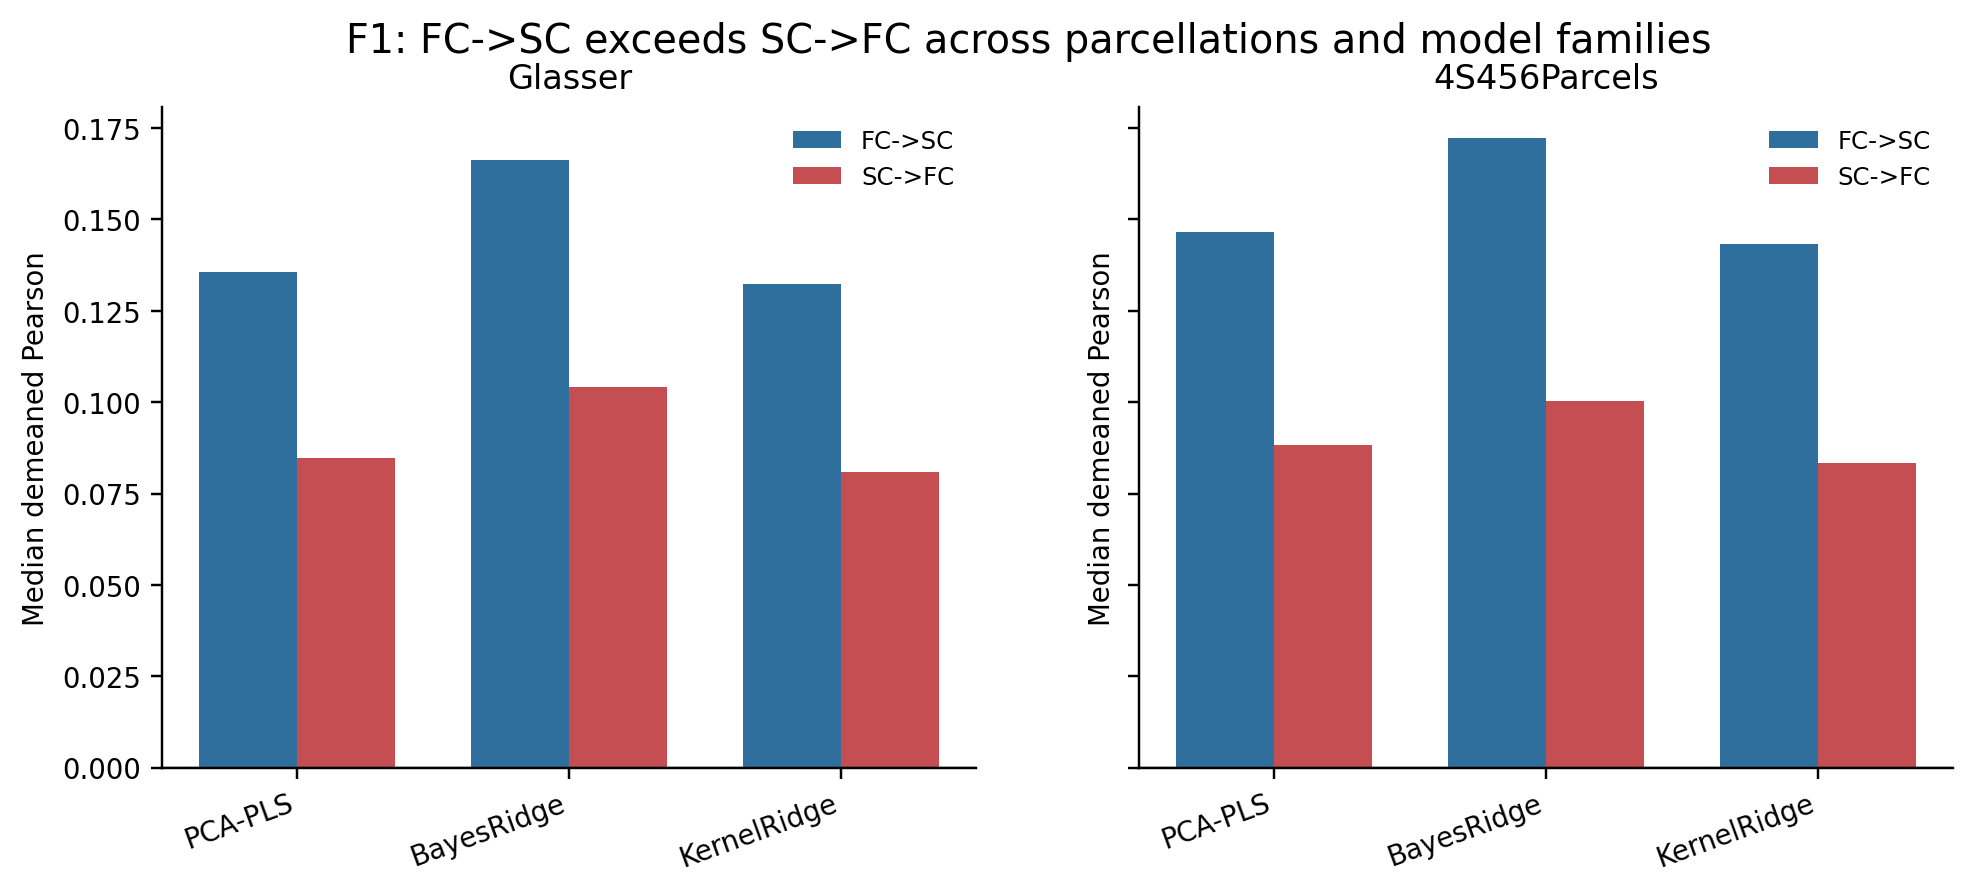
\includegraphics[width=0.95\linewidth]{figures/f1_asymmetry_models.png}
\caption{F1 across parcellations and model families. Bars show median demeaned Pearson for FC->SC and SC->FC. The FC->SC bar is higher in both atlases and across PCA-PLS, Bayesian ridge, and the kernel-ridge sweep.}
\label{fig:f1}
\end{figure}

\begin{table}[H]
\centering
\scriptsize
\caption{F1 median reconstruction metrics by parcellation and model family.}
\label{tab:f1}
\begin{tabular}{lllll}
\toprule
parcellation & model & FC->SC & SC->FC & ratio\_FC\_to\_SC\_over\_SC\_to\_FC \\
\midrule
4S456Parcels & BayesRidge & 0.172 & 0.100 & 1.715 \\
4S456Parcels & KernelRidge & 0.143 & 0.083 & 1.723 \\
4S456Parcels & PCA-PLS & 0.146 & 0.088 & 1.660 \\
Glasser & BayesRidge & 0.166 & 0.104 & 1.596 \\
Glasser & KernelRidge & 0.132 & 0.081 & 1.633 \\
Glasser & PCA-PLS & 0.135 & 0.085 & 1.600 \\
\bottomrule
\end{tabular}
\end{table}

The 4S456 parcellation gives slightly higher structure-target prediction and the Glasser
atlas gives nearly the same asymmetry ratio. This matters because the atlas comparison is
within-cohort and split-matched. The finer atlas does not invent the effect; it shifts the
absolute structural resolution while preserving the direction.  Sources: reproduction/outputs/reconstruction.csv; reproduction/reports/reproduction\_findings.md; reproduction/exploration/FINDINGS\_EXPLORATION.md; notebooks-FC\_to\_SC-experimental/sanity\_checks/preprocessing\_check/reduction\_axis\_summary.csv; notebooks-FC\_to\_SC-experimental/sanity\_checks/preprocessing\_check/findings.md.

\section{F2: Anatomy Predicts SC, Demographics Predict FC}

\textbf{Status: replicated on both parcellations.} F2 is a crossed dissociation, not a
single nuisance observation. Brain-volume/anatomy variables better predict structural
connectivity, while demographics better predict functional connectivity. The clean way to
write it is as a 2x2: anatomy has its natural target in SC; demographics have their
natural target in FC. The same family-aware split logic and model families are used.

\begin{figure}[H]
\centering
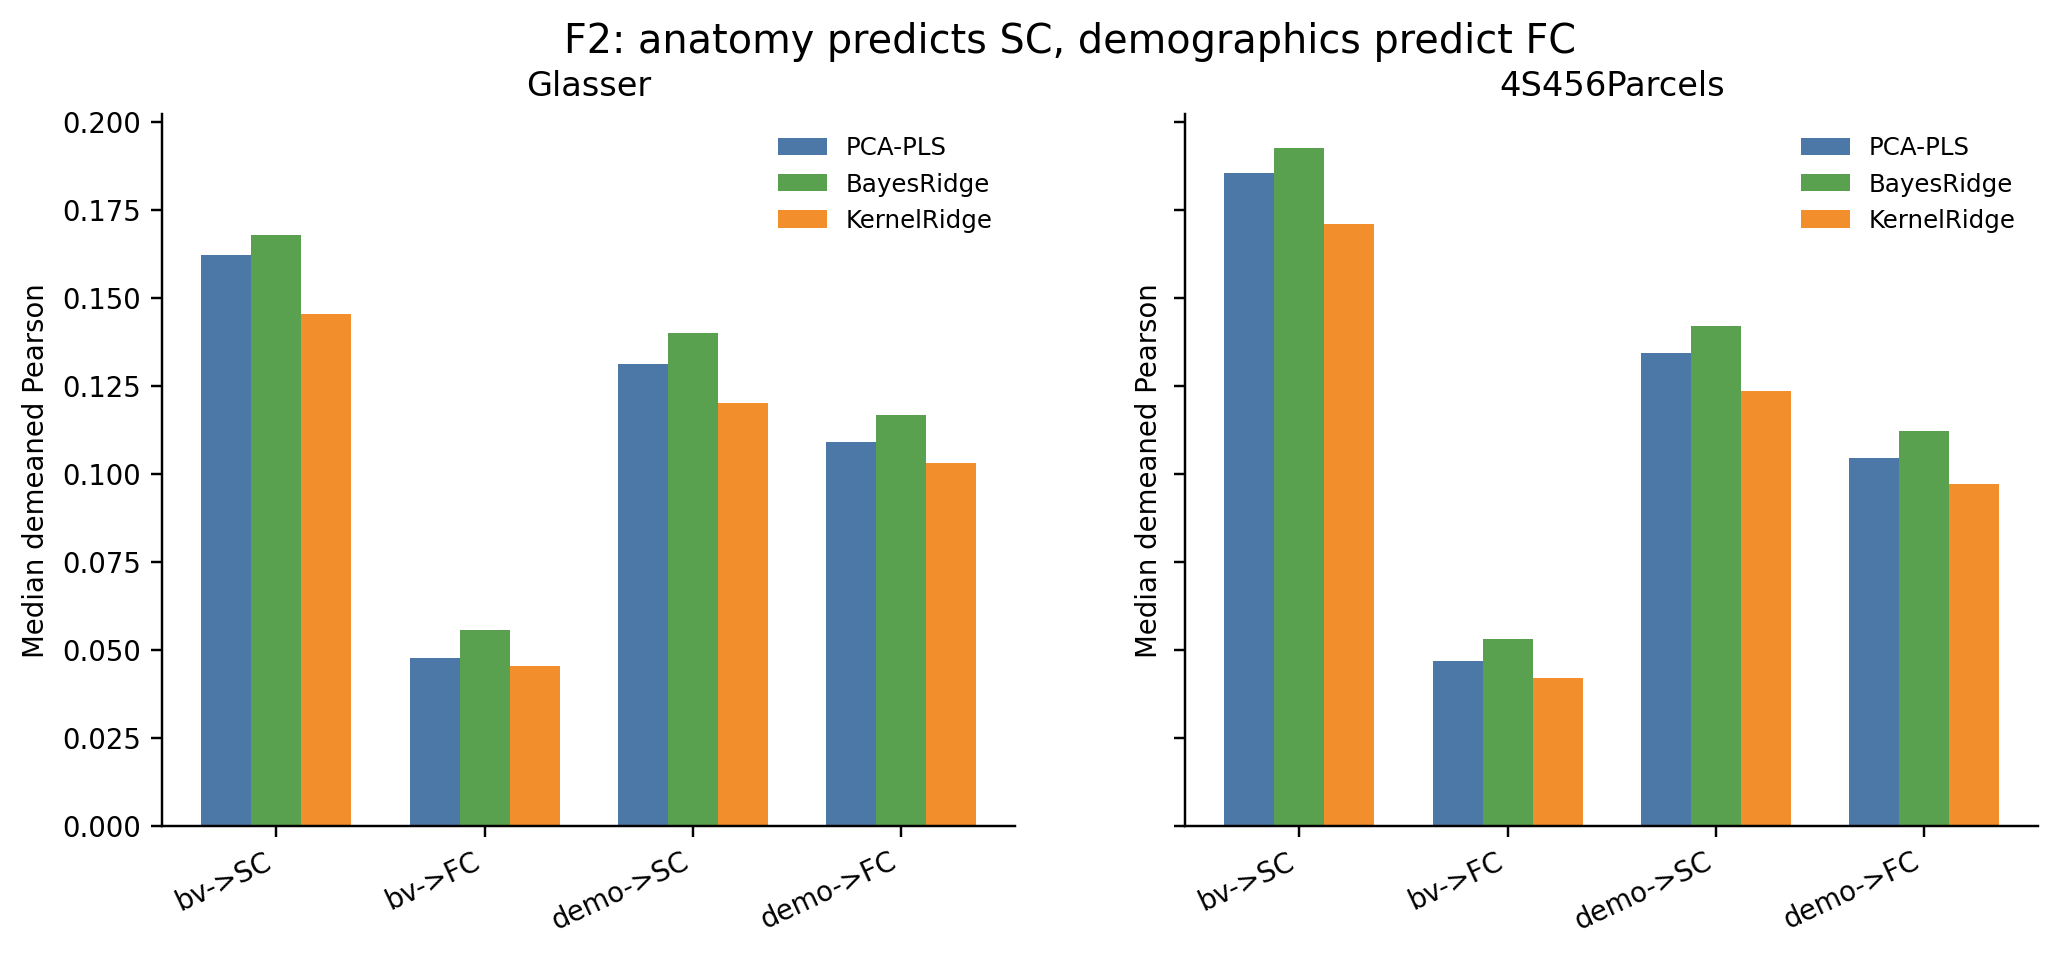
\includegraphics[width=0.95\linewidth]{figures/f2_double_dissociation_models.png}
\caption{F2 across parcellations and model families. Anatomy/brain-volume predicts SC more strongly than FC, while demographics shift toward FC. The crossover is visible in both atlases.}
\label{fig:f2}
\end{figure}

\begin{table}[H]
\centering
\scriptsize
\caption{F2 model ledger: source variables to structural or functional targets. Showing first 18 rows.}
\label{tab:f2}
\begin{tabular}{llllll}
\toprule
parcellation & model & direction & demeaned\_pearson & avg\_rank & top1\_acc \\
\midrule
4S456Parcels & BayesRidge & bv->FC & 0.053 & 0.658 & 0.015 \\
4S456Parcels & BayesRidge & bv->SC & 0.193 & 0.902 & 0.108 \\
4S456Parcels & BayesRidge & demo->FC & 0.112 & 0.673 & 0.015 \\
4S456Parcels & BayesRidge & demo->SC & 0.142 & 0.784 & 0.026 \\
4S456Parcels & KernelRidge & bv->FC & 0.042 & 0.612 & 0.013 \\
4S456Parcels & KernelRidge & bv->SC & 0.171 & 0.887 & 0.103 \\
4S456Parcels & KernelRidge & demo->FC & 0.097 & 0.666 & 0.015 \\
4S456Parcels & KernelRidge & demo->SC & 0.124 & 0.738 & 0.021 \\
4S456Parcels & PCA-PLS & bv->FC & 0.047 & 0.626 & 0.010 \\
4S456Parcels & PCA-PLS & bv->SC & 0.185 & 0.904 & 0.128 \\
4S456Parcels & PCA-PLS & demo->FC & 0.105 & 0.673 & 0.013 \\
4S456Parcels & PCA-PLS & demo->SC & 0.134 & 0.769 & 0.026 \\
Glasser & BayesRidge & bv->FC & 0.055 & 0.651 & 0.013 \\
Glasser & BayesRidge & bv->SC & 0.168 & 0.867 & 0.077 \\
Glasser & BayesRidge & demo->FC & 0.117 & 0.664 & 0.013 \\
Glasser & BayesRidge & demo->SC & 0.140 & 0.767 & 0.020 \\
Glasser & KernelRidge & bv->FC & 0.045 & 0.618 & 0.010 \\
Glasser & KernelRidge & bv->SC & 0.146 & 0.843 & 0.069 \\
\bottomrule
\end{tabular}
\end{table}

The dissociation is central because it turns bv+demo from a nuisance into a required
scientific baseline. A connectome that cannot beat cheap subject-level covariates should
not be advertised as a useful cognitive biomarker.  Sources: reproduction/outputs/reconstruction.csv; reproduction/exploration/FINDINGS\_EXPLORATION.md; notebooks-FC\_to\_SC-experimental/MASTER\_FINDINGS.md.

\section{F3: Imputed Connectomes Are Usable, But Utility Is Asymmetric}

\textbf{Status: replicated on both parcellations, interpreted through F5.} F3 is the
bridge between reconstruction and downstream utility. Predicted connectomes are not
random. They carry source-modality information and can support some downstream tasks. But
the utility is not symmetric: imputed SC from FC is closer to neutral or mildly useful,
whereas imputed FC from SC is often harmful for cognition. This is why the paper should
not stop at reconstruction metrics.

\begin{figure}[H]
\centering
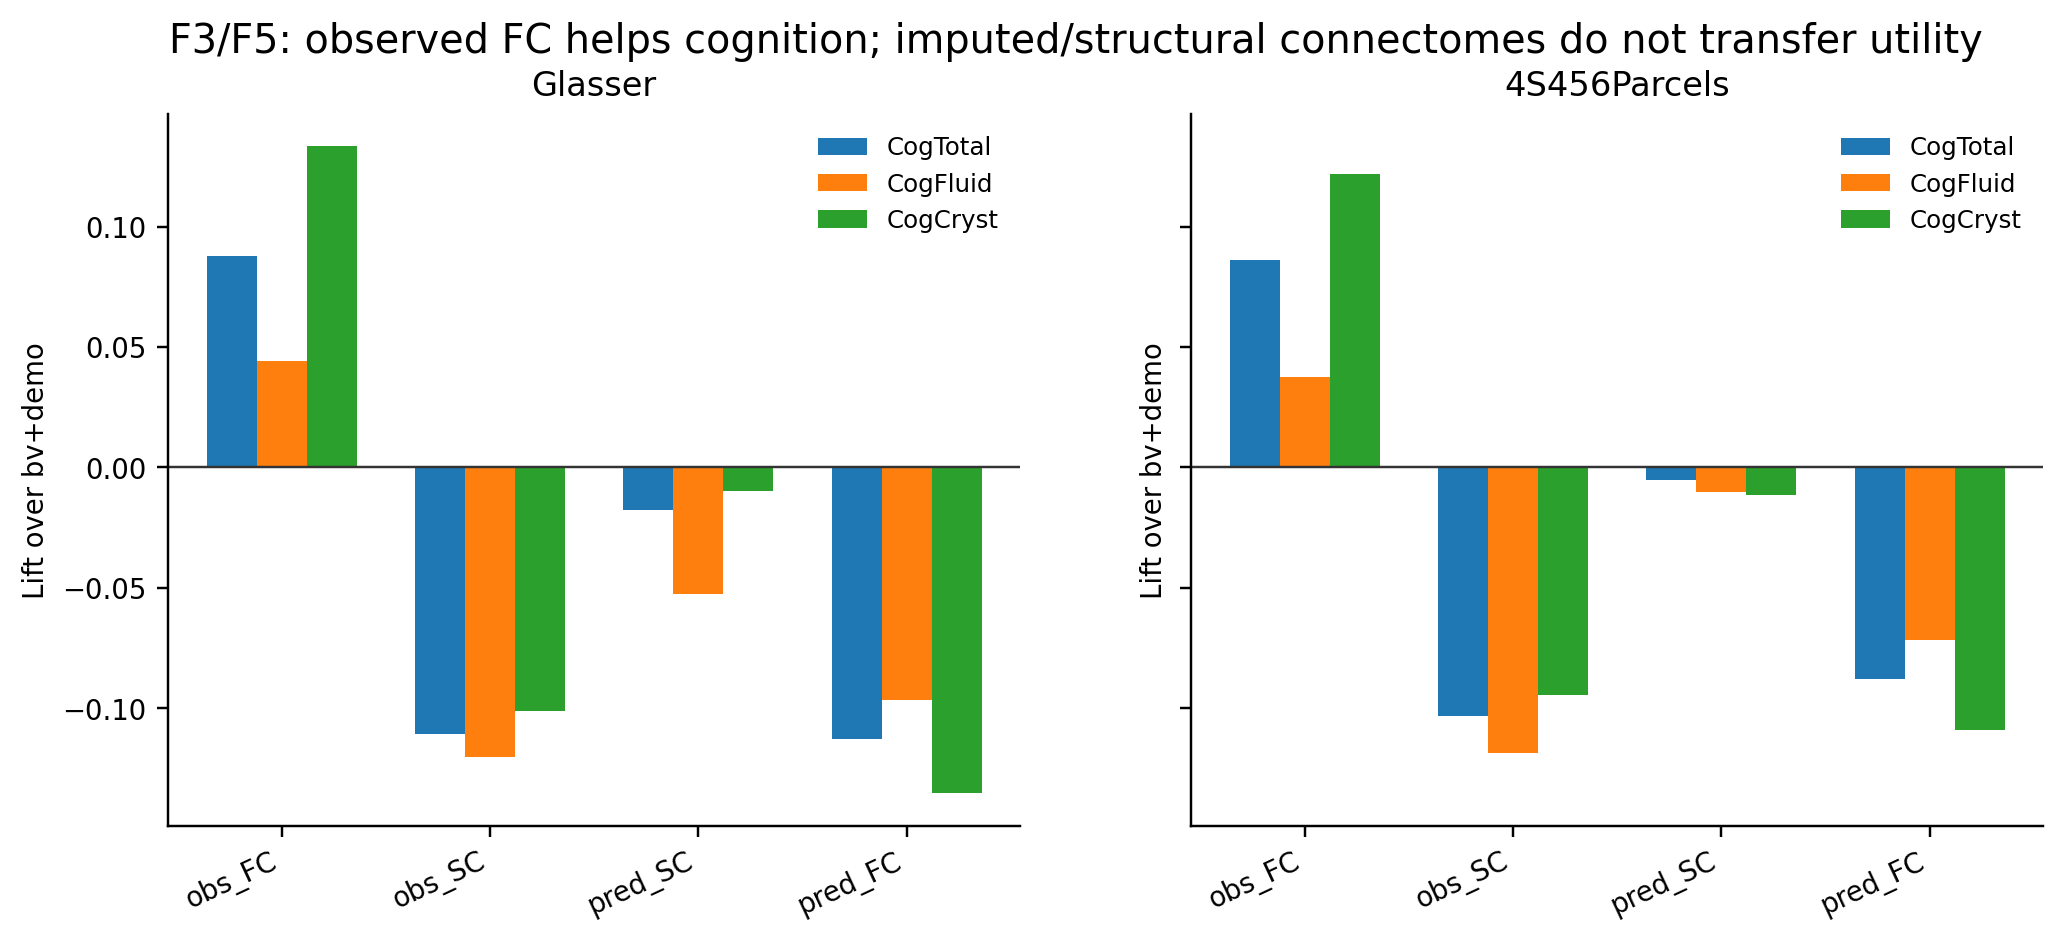
\includegraphics[width=0.95\linewidth]{figures/f3_f5_imputation_utility.png}
\caption{F3/F5 downstream utility ledger. Bayesian-ridge cognition lift over bv+demo is shown for observed and predicted FC/SC. Observed FC carries the positive signal; structural and imputed representations do not transfer it reliably.}
\label{fig:f3}
\end{figure}

\begin{table}[H]
\centering
\scriptsize
\caption{F3 downstream utility of observed and imputed connectomes, Bayesian ridge. Showing first 18 rows.}
\label{tab:f3}
\begin{tabular}{lllllll}
\toprule
parcellation & input\_set & target & pearson & lift\_over\_bvdemo & median\_perm\_p & residualized\_pearson \\
\midrule
4S456Parcels & obs\_FC & CogCryst & 0.476 & 0.122 & 0.041 & 0.352 \\
4S456Parcels & obs\_SC & CogCryst & 0.259 & -0.095 & 0.883 & 0.066 \\
4S456Parcels & pred\_FC & CogCryst & 0.245 & -0.109 & 0.896 & 0.025 \\
4S456Parcels & pred\_SC & CogCryst & 0.342 & -0.012 & 0.629 & 0.184 \\
4S456Parcels & obs\_FC & CogFluid & 0.321 & 0.037 & 0.347 & 0.204 \\
4S456Parcels & obs\_SC & CogFluid & 0.165 & -0.118 & 0.971 & 0.030 \\
4S456Parcels & pred\_FC & CogFluid & 0.211 & -0.072 & 0.906 & 0.091 \\
4S456Parcels & pred\_SC & CogFluid & 0.273 & -0.010 & 0.843 & 0.152 \\
4S456Parcels & obs\_FC & CogTotal & 0.445 & 0.086 & 0.090 & 0.289 \\
4S456Parcels & obs\_SC & CogTotal & 0.256 & -0.103 & 0.927 & 0.057 \\
4S456Parcels & pred\_FC & CogTotal & 0.271 & -0.088 & 0.871 & 0.079 \\
4S456Parcels & pred\_SC & CogTotal & 0.354 & -0.005 & 0.612 & 0.182 \\
Glasser & obs\_FC & CogCryst & 0.487 & 0.133 & 0.031 & 0.378 \\
Glasser & obs\_SC & CogCryst & 0.253 & -0.101 & 0.817 & 0.061 \\
Glasser & pred\_FC & CogCryst & 0.219 & -0.135 & 0.960 & -7.69e-05 \\
Glasser & pred\_SC & CogCryst & 0.344 & -0.010 & 0.582 & 0.195 \\
Glasser & obs\_FC & CogFluid & 0.327 & 0.044 & 0.326 & 0.216 \\
Glasser & obs\_SC & CogFluid & 0.163 & -0.120 & 0.977 & 0.008 \\
\bottomrule
\end{tabular}
\end{table}

The model caveat is important. The scalar downstream grid includes PCA-PLS and kernel
ridge rows, but the project ledger treats Bayesian ridge as the reportable scalar
estimator because the discrepancy audit showed it is stable for cognition targets. The
other model families are still useful as sensitivity checks; they do not rescue the
imputation story.  Sources: reproduction/outputs/downstream.csv; reproduction/exploration/FINDINGS\_EXPLORATION.md; reproduction/reports/reproduction\_findings.md.

\section{F4: Observed FC Carries Real Cognition Signal}

\textbf{Status: replicated on both parcellations.} F4 is the positive control for the
entire cognition argument. If the pipeline could not detect any connectome-cognition
signal at all, the SC/imputation null would be much less meaningful. Observed FC does
clear the bv+demo floor, especially for crystallized cognition. This gives the negative
claims teeth: the downstream framework can find signal when signal exists.

\begin{figure}[H]
\centering
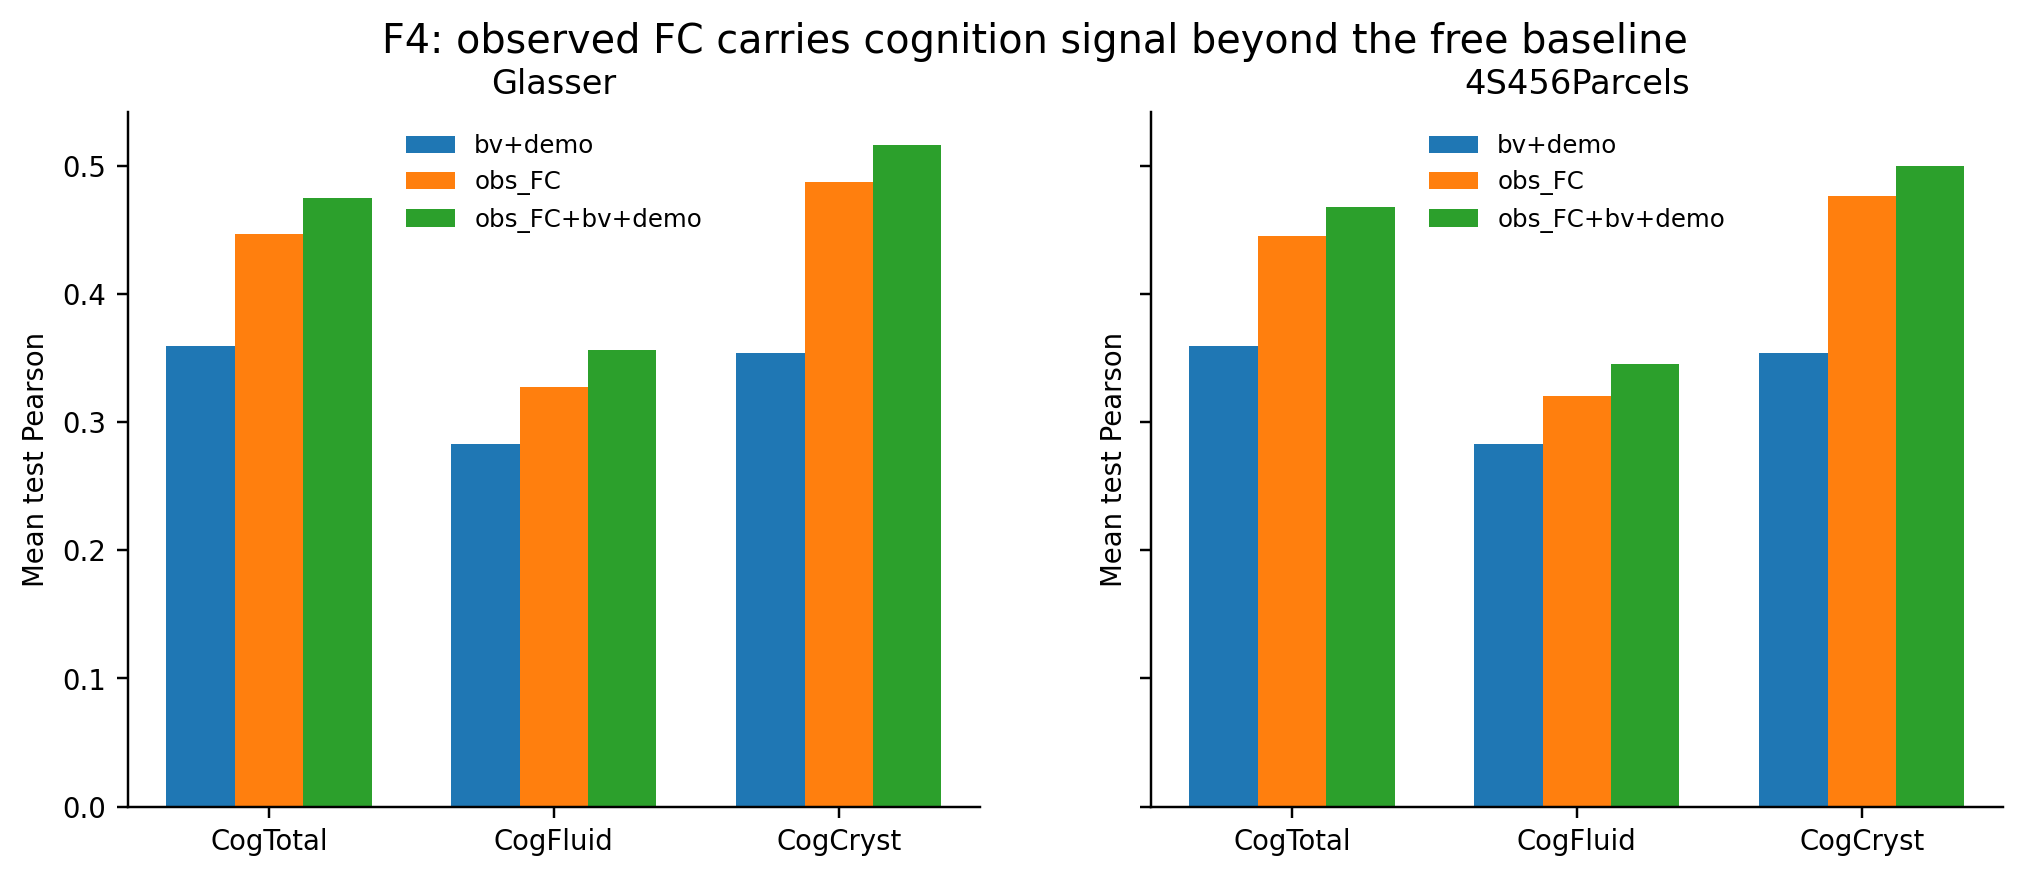
\includegraphics[width=0.95\linewidth]{figures/f4_observed_fc_cognition.png}
\caption{F4 observed FC cognition signal. Mean Bayesian-ridge Pearson is shown for bv+demo, observed FC, and observed FC plus bv+demo across cognition targets and parcellations.}
\label{fig:f4}
\end{figure}

\begin{table}[H]
\centering
\scriptsize
\caption{F4 observed FC vs bv+demo cognition ledger.}
\label{tab:f4}
\begin{tabular}{lllllll}
\toprule
parcellation & input\_set & target & pearson & lift\_over\_bvdemo & median\_perm\_p & residualized\_pearson \\
\midrule
4S456Parcels & bv+demo & CogCryst & 0.354 & 0.000 & 1.000 & 0.054 \\
4S456Parcels & obs\_FC & CogCryst & 0.476 & 0.122 & 0.041 & 0.352 \\
4S456Parcels & obs\_FC+bv+demo & CogCryst & 0.500 & 0.146 & 0.008 & 0.353 \\
4S456Parcels & bv+demo & CogFluid & 0.283 & 0.000 & 1.000 & -0.003 \\
4S456Parcels & obs\_FC & CogFluid & 0.321 & 0.037 & 0.347 & 0.204 \\
4S456Parcels & obs\_FC+bv+demo & CogFluid & 0.345 & 0.062 & 0.158 & 0.208 \\
4S456Parcels & bv+demo & CogTotal & 0.359 & 0.000 & 1.000 & 0.022 \\
4S456Parcels & obs\_FC & CogTotal & 0.445 & 0.086 & 0.090 & 0.289 \\
4S456Parcels & obs\_FC+bv+demo & CogTotal & 0.468 & 0.109 & 0.019 & 0.292 \\
Glasser & bv+demo & CogCryst & 0.354 & 0.000 & 1.000 & 0.054 \\
Glasser & obs\_FC & CogCryst & 0.487 & 0.133 & 0.031 & 0.378 \\
Glasser & obs\_FC+bv+demo & CogCryst & 0.516 & 0.162 & 0.002 & 0.382 \\
Glasser & bv+demo & CogFluid & 0.283 & 0.000 & 1.000 & -0.003 \\
Glasser & obs\_FC & CogFluid & 0.327 & 0.044 & 0.326 & 0.216 \\
Glasser & obs\_FC+bv+demo & CogFluid & 0.356 & 0.073 & 0.095 & 0.219 \\
Glasser & bv+demo & CogTotal & 0.359 & 0.000 & 1.000 & 0.022 \\
Glasser & obs\_FC & CogTotal & 0.447 & 0.088 & 0.080 & 0.297 \\
Glasser & obs\_FC+bv+demo & CogTotal & 0.474 & 0.115 & 0.016 & 0.303 \\
\bottomrule
\end{tabular}
\end{table}

The result is intentionally modest. These are research-grade correlations, not a clinical
biomarker. The point is comparative: FC is the modality that adds cognitive information
above the cheap floor in this dataset; SC does not.  Sources: reproduction/outputs/downstream.csv; notebooks-FC\_to\_SC-experimental/MASTER\_FINDINGS.md; reproduction/exploration/FINDINGS\_EXPLORATION.md.

\section{F5: SC Underperforms, Imputation Does Not Transfer Cognition Utility}

\textbf{Status: replicated on both parcellations.} F5 is the paper's main redirect.
Observed SC is below the bv+demo floor for cognition, predicted SC is at best small and
target-dependent, and predicted FC is often actively harmful. This is stronger than
"imputation is useless." It says reconstruction can manufacture a plausible connectome
whose downstream cognitive content is misaligned with what real FC carries.

\begin{figure}[H]
\centering
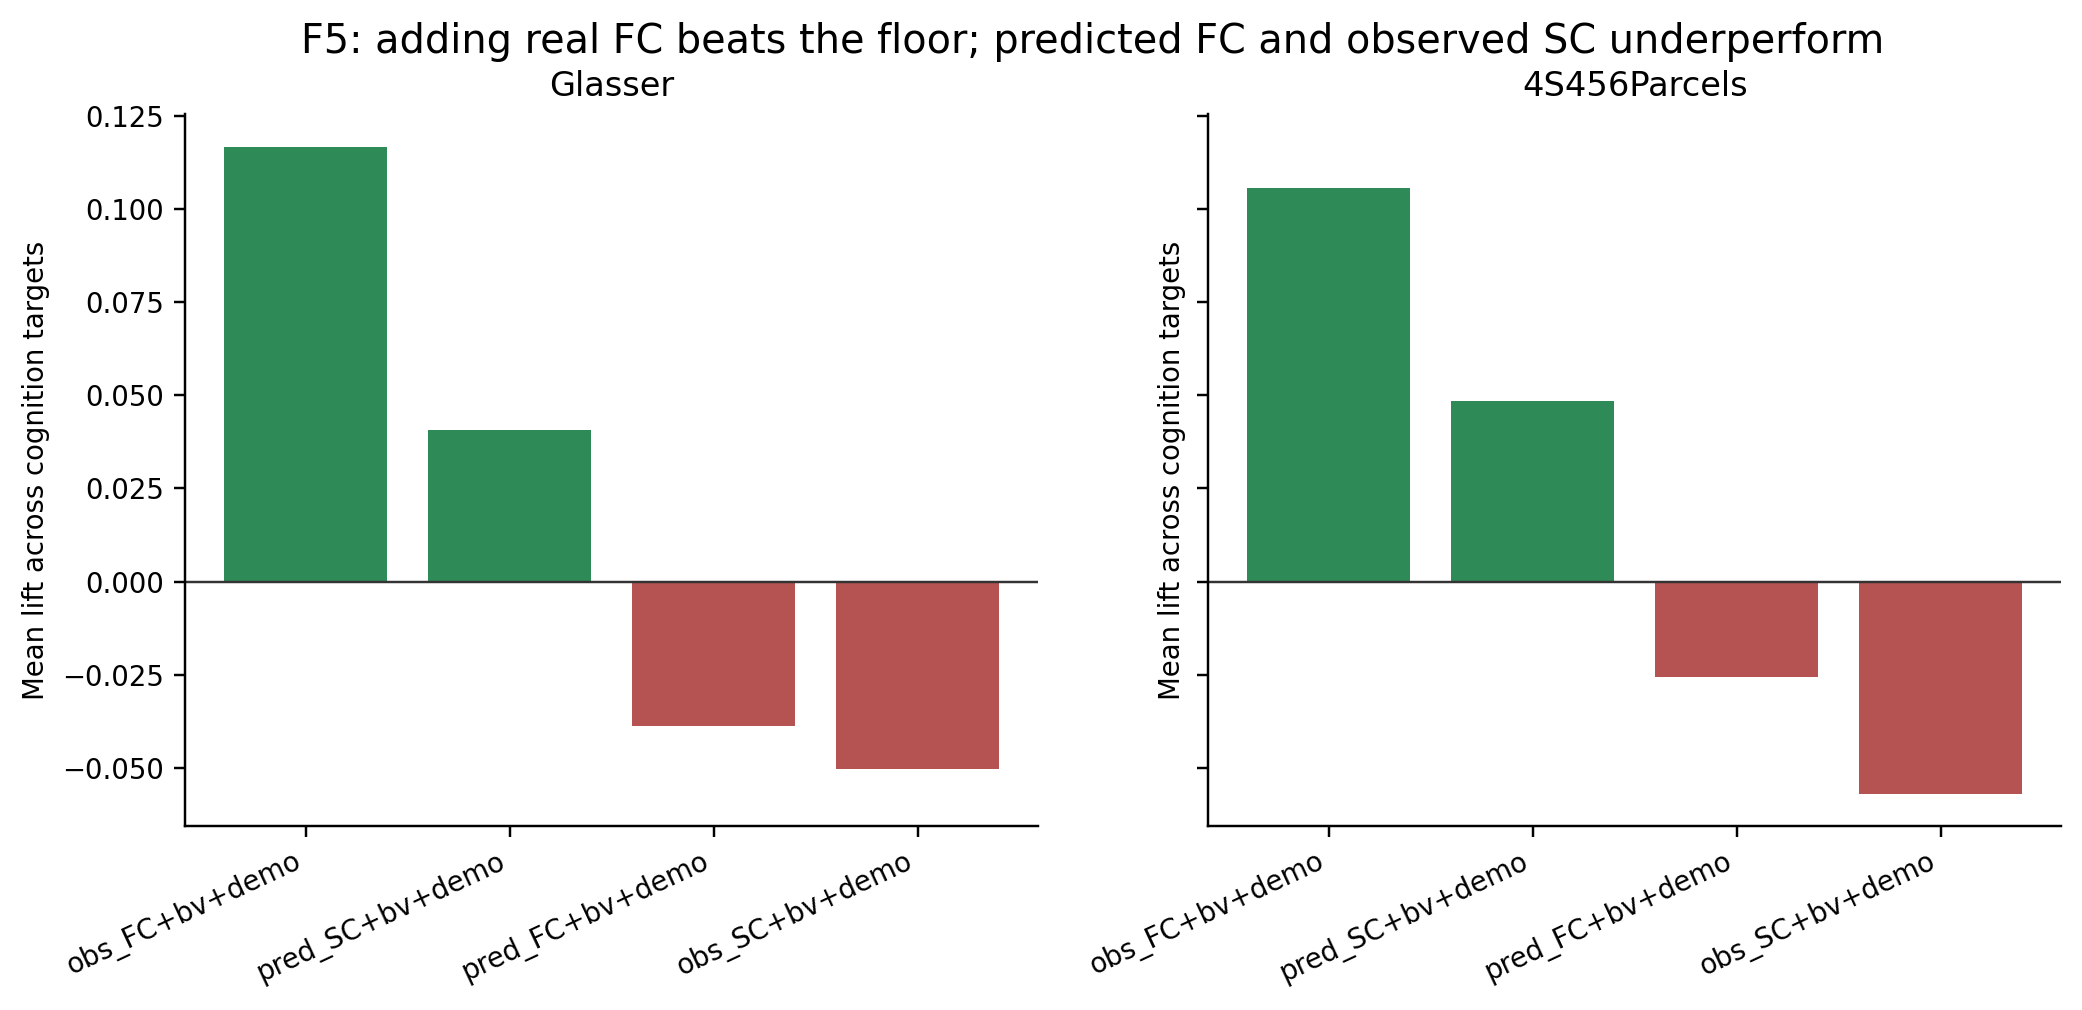
\includegraphics[width=0.95\linewidth]{figures/f5_sc_predfc_underperform.png}
\caption{F5 cognition lift when each connectome is added to bv+demo. Observed FC gives a positive lift; predicted SC is smaller; predicted FC and observed SC underperform.}
\label{fig:f5}
\end{figure}

\begin{table}[H]
\centering
\scriptsize
\caption{F5 connectome plus bv+demo cognition ledger, Bayesian ridge. Showing first 18 rows.}
\label{tab:f5}
\begin{tabular}{llllll}
\toprule
parcellation & input\_set & target & pearson & lift\_over\_bvdemo & median\_perm\_p \\
\midrule
4S456Parcels & obs\_FC+bv+demo & CogCryst & 0.500 & 0.146 & 0.008 \\
4S456Parcels & obs\_SC+bv+demo & CogCryst & 0.312 & -0.042 & 0.695 \\
4S456Parcels & pred\_FC+bv+demo & CogCryst & 0.326 & -0.028 & 0.542 \\
4S456Parcels & pred\_SC+bv+demo & CogCryst & 0.410 & 0.056 & 0.048 \\
4S456Parcels & obs\_FC+bv+demo & CogFluid & 0.345 & 0.062 & 0.158 \\
4S456Parcels & obs\_SC+bv+demo & CogFluid & 0.206 & -0.077 & 0.934 \\
4S456Parcels & pred\_FC+bv+demo & CogFluid & 0.260 & -0.024 & 0.765 \\
4S456Parcels & pred\_SC+bv+demo & CogFluid & 0.325 & 0.042 & 0.216 \\
4S456Parcels & obs\_FC+bv+demo & CogTotal & 0.468 & 0.109 & 0.019 \\
4S456Parcels & obs\_SC+bv+demo & CogTotal & 0.308 & -0.052 & 0.831 \\
4S456Parcels & pred\_FC+bv+demo & CogTotal & 0.334 & -0.025 & 0.735 \\
4S456Parcels & pred\_SC+bv+demo & CogTotal & 0.407 & 0.048 & 0.143 \\
Glasser & obs\_FC+bv+demo & CogCryst & 0.516 & 0.162 & 0.002 \\
Glasser & obs\_SC+bv+demo & CogCryst & 0.319 & -0.035 & 0.604 \\
Glasser & pred\_FC+bv+demo & CogCryst & 0.314 & -0.040 & 0.813 \\
Glasser & pred\_SC+bv+demo & CogCryst & 0.415 & 0.061 & 0.037 \\
Glasser & obs\_FC+bv+demo & CogFluid & 0.356 & 0.073 & 0.095 \\
Glasser & obs\_SC+bv+demo & CogFluid & 0.217 & -0.066 & 0.937 \\
\bottomrule
\end{tabular}
\end{table}

This section should be written as an objective mismatch, not a model failure. F6 and F7
show why: predicted connectomes can carry real biological/family signal, but the signal
selected by reconstruction is not the one needed for cognition.  Sources: reproduction/outputs/downstream.csv; reproduction/exploration/FINDINGS\_EXPLORATION.md; reproduction/outputs/leak\_verdict.csv.

\section{F6: Predicted Connectomes Carry Heritable Family Signal}

\textbf{Status: replicated on both parcellations.} F6 prevents an over-simple reading of
F5. Predicted connectomes are not empty artifacts. When the analysis asks whether they
preserve family structure, the answer is yes. The strongest sibling result is the
predicted SC residualized against bv+demo, which separates siblings from unrelated pairs
well above the bv+demo-only baseline in both parcellations.

\begin{figure}[H]
\centering
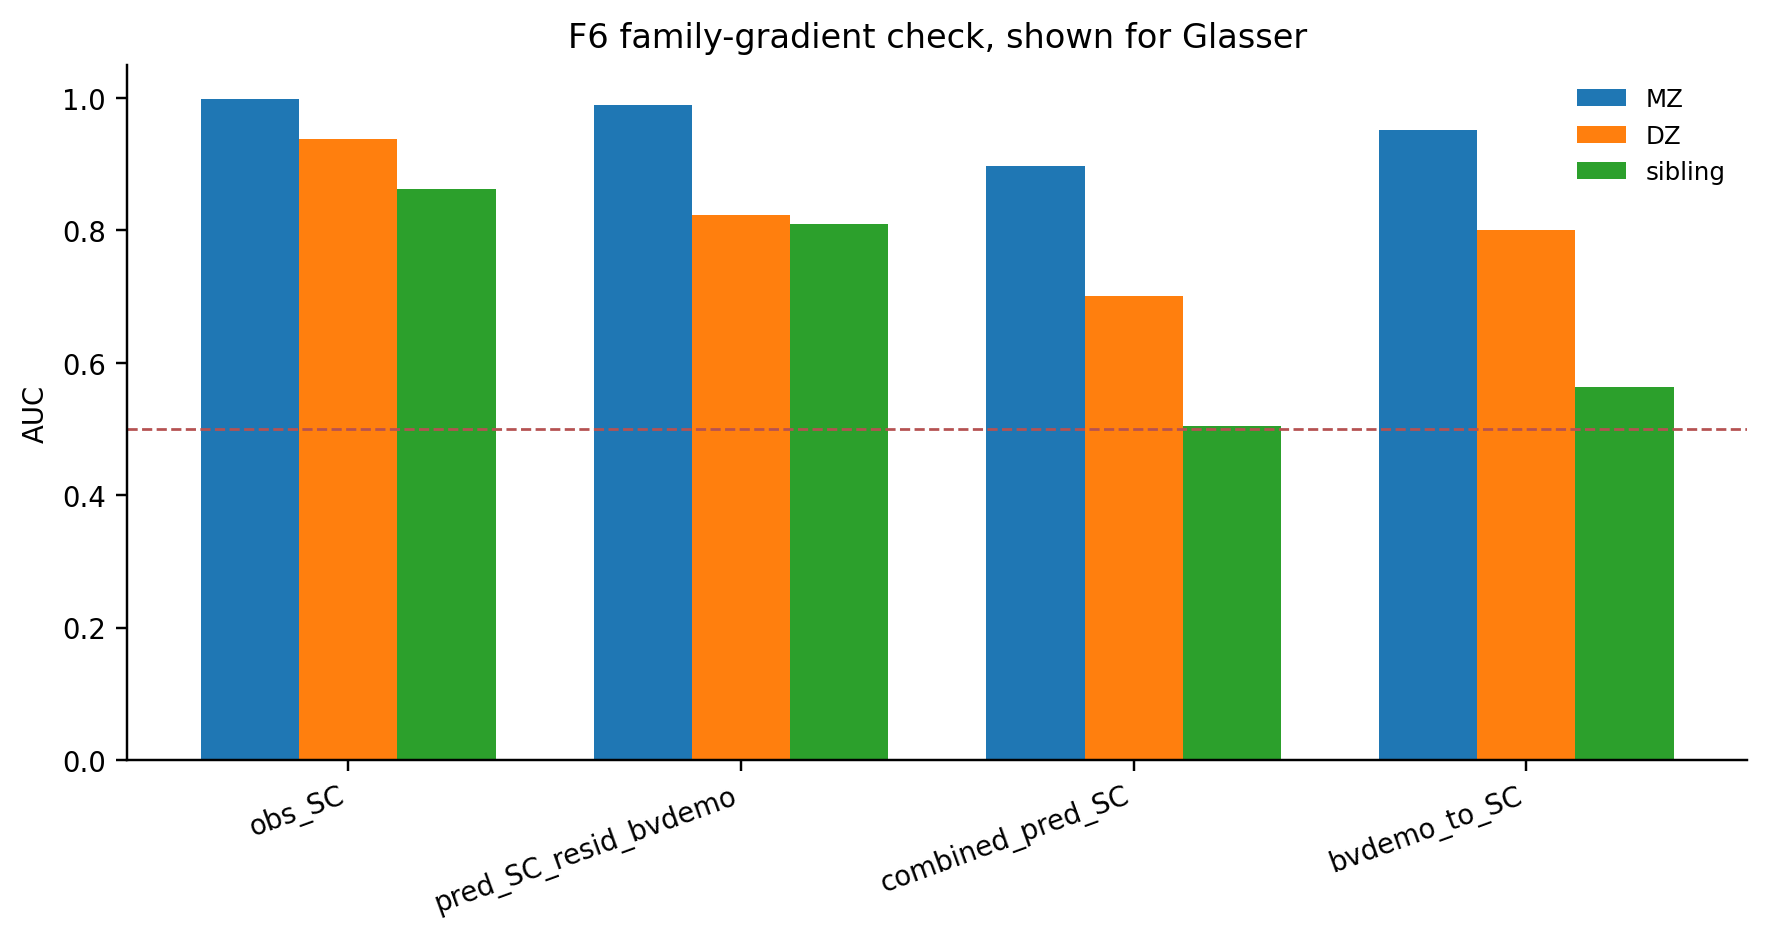
\includegraphics[width=0.95\linewidth]{figures/f6_family_gradient.png}
\caption{F6 family-gradient check. AUCs are shown for MZ, DZ, and sibling separation in selected variants. Predicted SC residualized against bv+demo preserves family signal beyond the subject-info baseline.}
\label{fig:f6}
\end{figure}

\begin{table}[H]
\centering
\scriptsize
\caption{F6 family AUCs with confidence intervals and FDR-adjusted permutation tests.}
\label{tab:f6}
\begin{tabular}{llllllll}
\toprule
parcellation & variant & relation & auc & auc\_lo & auc\_hi & p\_fdr & sig\_fdr \\
\midrule
4S456Parcels & bvdemo\_to\_SC & DZ & 0.791 & 0.748 & 0.831 & 0.000 & yes \\
4S456Parcels & bvdemo\_to\_SC & MZ & 0.949 & 0.934 & 0.964 & 0.000 & yes \\
4S456Parcels & bvdemo\_to\_SC & sibling & 0.565 & 0.544 & 0.586 & 0.000 & yes \\
4S456Parcels & obs\_FC & DZ & 0.886 & 0.851 & 0.916 & 0.000 & yes \\
4S456Parcels & obs\_FC & MZ & 0.991 & 0.986 & 0.995 & 0.000 & yes \\
4S456Parcels & obs\_FC & sibling & 0.821 & 0.805 & 0.836 & 0.000 & yes \\
4S456Parcels & obs\_SC & DZ & 0.958 & 0.946 & 0.968 & 0.000 & yes \\
4S456Parcels & obs\_SC & MZ & 0.999 & 0.999 & 1.000 & 0.000 & yes \\
4S456Parcels & obs\_SC & sibling & 0.884 & 0.873 & 0.896 & 0.000 & yes \\
4S456Parcels & pred\_SC\_resid\_bvdemo & DZ & 0.847 & 0.810 & 0.880 & 0.000 & yes \\
4S456Parcels & pred\_SC\_resid\_bvdemo & MZ & 0.994 & 0.991 & 0.997 & 0.000 & yes \\
4S456Parcels & pred\_SC\_resid\_bvdemo & sibling & 0.816 & 0.801 & 0.831 & 0.000 & yes \\
Glasser & bvdemo\_to\_SC & DZ & 0.800 & 0.759 & 0.840 & 0.000 & yes \\
Glasser & bvdemo\_to\_SC & MZ & 0.951 & 0.935 & 0.964 & 0.000 & yes \\
Glasser & bvdemo\_to\_SC & sibling & 0.563 & 0.541 & 0.585 & 0.000 & yes \\
Glasser & obs\_FC & DZ & 0.886 & 0.852 & 0.914 & 0.000 & yes \\
Glasser & obs\_FC & MZ & 0.990 & 0.984 & 0.994 & 0.000 & yes \\
Glasser & obs\_FC & sibling & 0.823 & 0.807 & 0.839 & 0.000 & yes \\
Glasser & obs\_SC & DZ & 0.938 & 0.924 & 0.951 & 0.000 & yes \\
Glasser & obs\_SC & MZ & 0.999 & 0.998 & 1.000 & 0.000 & yes \\
Glasser & obs\_SC & sibling & 0.863 & 0.850 & 0.876 & 0.000 & yes \\
Glasser & pred\_SC\_resid\_bvdemo & DZ & 0.823 & 0.784 & 0.860 & 0.000 & yes \\
Glasser & pred\_SC\_resid\_bvdemo & MZ & 0.989 & 0.982 & 0.994 & 0.000 & yes \\
Glasser & pred\_SC\_resid\_bvdemo & sibling & 0.810 & 0.795 & 0.825 & 0.000 & yes \\
\bottomrule
\end{tabular}
\end{table}

The family result is constructive: cross-modal prediction can preserve a heritable
connectome signature. The lesson is narrower and more interesting than "prediction is
bad." Prediction preserves the signal selected by its objective and representation.
 Sources: reproduction/family\_mechanism/outputs/family\_auc.csv; dev-notes/PROJECT-HANDOFF-2026-06-22.md; notebooks-FC\_to\_SC-experimental/MASTER\_FINDINGS.md.

\section{F7: Reconstruction and Identification Objectives Trade Off}

\textbf{Status: replicated on both parcellations.} F7 is the objective warning. The
combined reconstruction-oriented predicted SC looks like a better reconstruction object,
but sibling identification collapses to chance. The residualized predicted SC keeps
family signal, while the combined reconstruction variant does not. Thus one cannot
assume that optimizing reconstruction, identification, and cognition are aligned.

\begin{figure}[H]
\centering
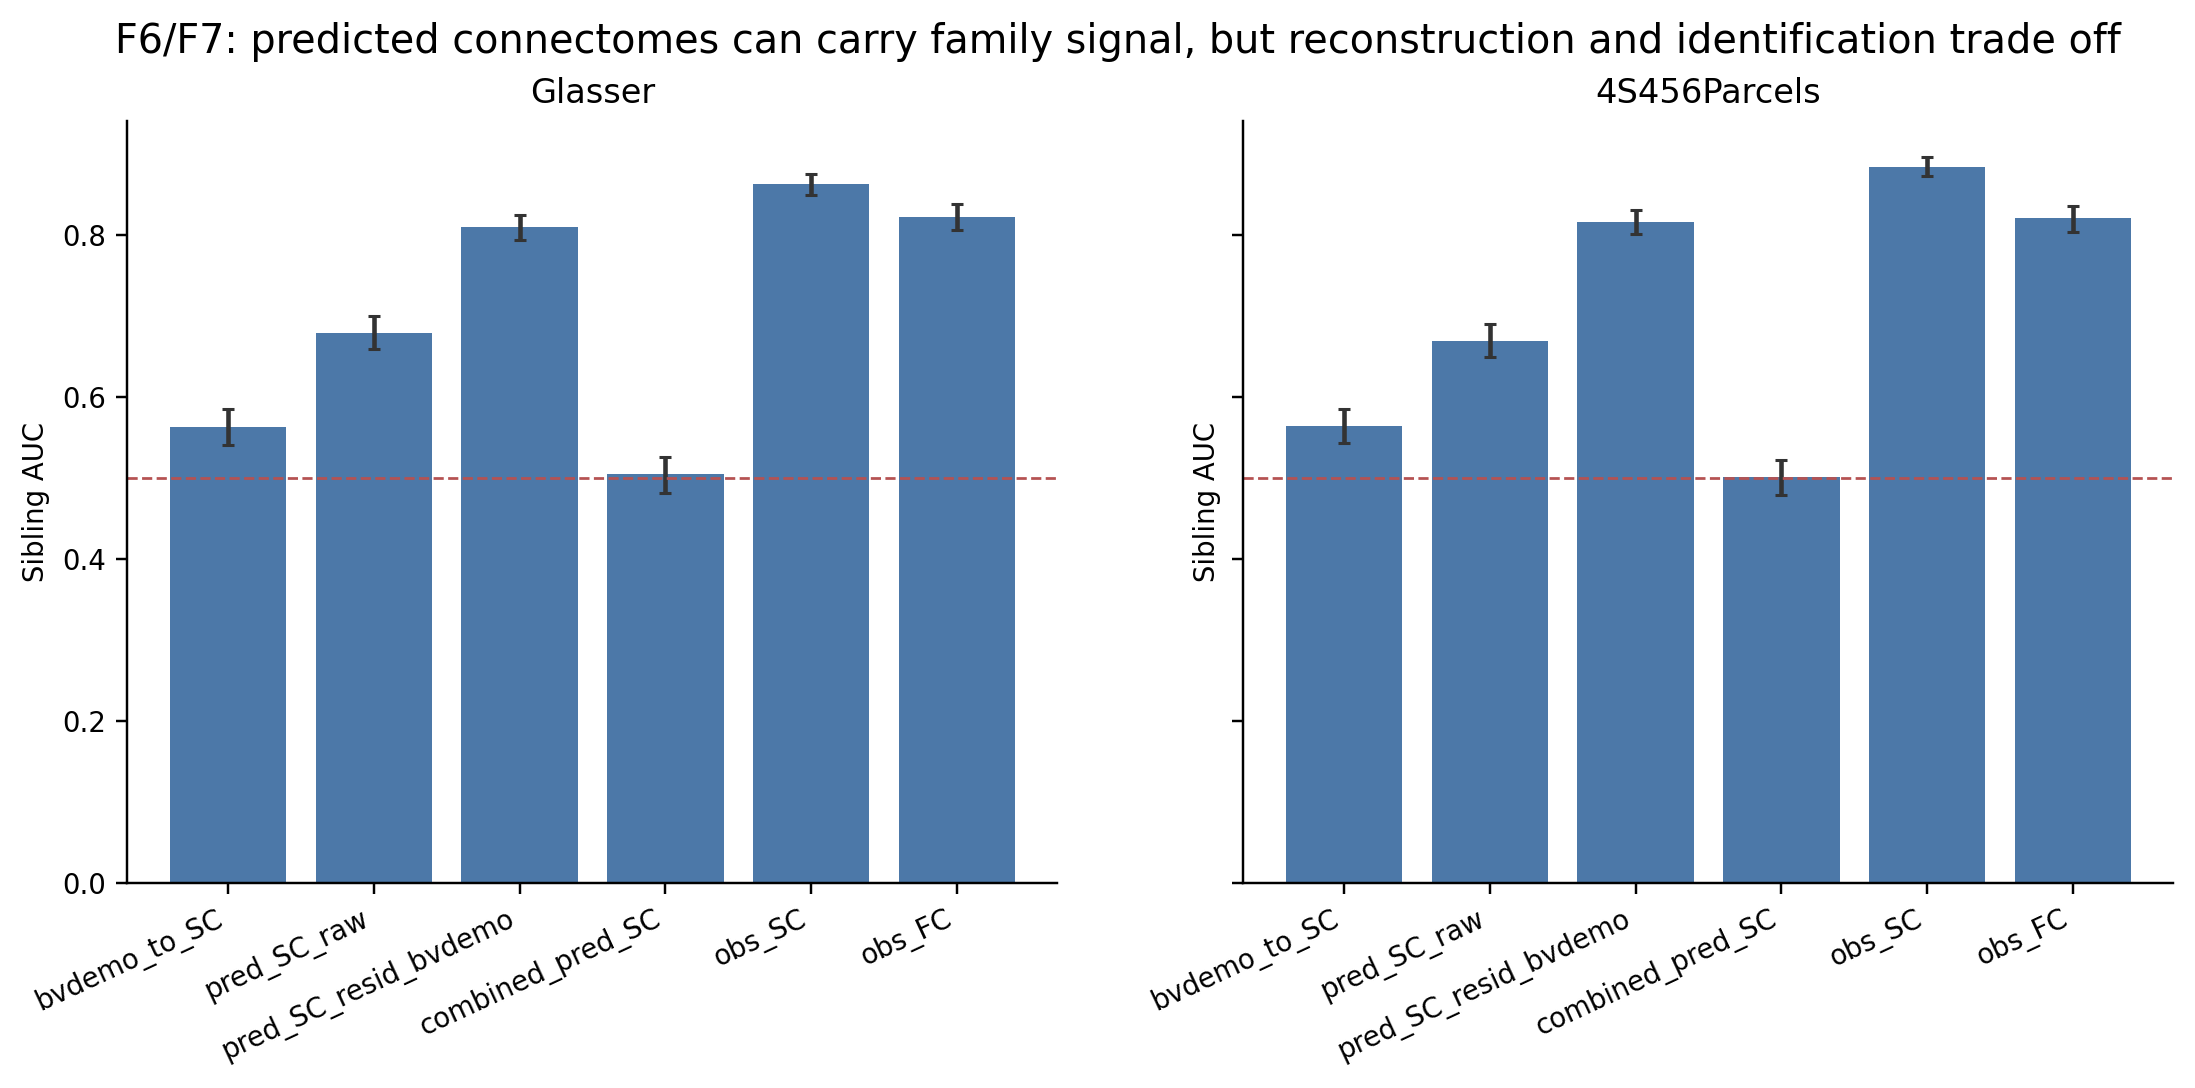
\includegraphics[width=0.95\linewidth]{figures/f6_f7_family_tradeoff.png}
\caption{F6/F7 sibling AUC across objective variants. The combined predicted SC variant collapses to chance for sibling separation, while pred\_SC\_resid\_bvdemo remains strongly above chance.}
\label{fig:f7}
\end{figure}

\begin{table}[H]
\centering
\scriptsize
\caption{F7 sibling AUC objective tradeoff.}
\label{tab:f7}
\begin{tabular}{lllllll}
\toprule
parcellation & variant & auc & auc\_lo & auc\_hi & p\_fdr & sig\_fdr \\
\midrule
4S456Parcels & bvdemo\_to\_SC & 0.565 & 0.544 & 0.586 & 0.000 & yes \\
4S456Parcels & combined\_pred\_SC & 0.501 & 0.479 & 0.523 & 0.904 & no \\
4S456Parcels & pred\_SC\_raw & 0.670 & 0.650 & 0.690 & 0.000 & yes \\
4S456Parcels & pred\_SC\_resid\_bvdemo & 0.816 & 0.801 & 0.831 & 0.000 & yes \\
Glasser & bvdemo\_to\_SC & 0.563 & 0.541 & 0.585 & 0.000 & yes \\
Glasser & combined\_pred\_SC & 0.505 & 0.482 & 0.526 & 0.648 & no \\
Glasser & pred\_SC\_raw & 0.680 & 0.660 & 0.700 & 0.000 & yes \\
Glasser & pred\_SC\_resid\_bvdemo & 0.810 & 0.795 & 0.825 & 0.000 & yes \\
\bottomrule
\end{tabular}
\end{table}

This is the best conceptual support for the manuscript's redirect: the missing cognition
transfer is not because the predicted connectomes are vacuous. It is because connectome
objectives are not interchangeable.  Sources: reproduction/family\_mechanism/outputs/family\_auc.csv; reproduction/exploration/FINDINGS\_EXPLORATION.md; notebooks-FC\_to\_SC-experimental/MASTER\_FINDINGS.md.

\section{F8: Exploratory PC Mechanism, PC3 Glasser / PC4 4S456}

\textbf{Status: partial and hypothesis-generating.} F8 should be written carefully. The
mechanism-like structural PC exists in the property sense: a low-variance SC mode is
moderately FC-predictable, carries weak family signal, and localizes to visual and dorsal
attention edges. But the index is atlas-sensitive: the Glasser story is PC3, while the
4S456 mechanism shifts to a neighboring PC. Therefore the right claim is not "PC3 is the
biomarker." The right claim is "there is a small, heritable, FC-predictable structural
mode whose exact PC index depends on the atlas."

\begin{figure}[H]
\centering
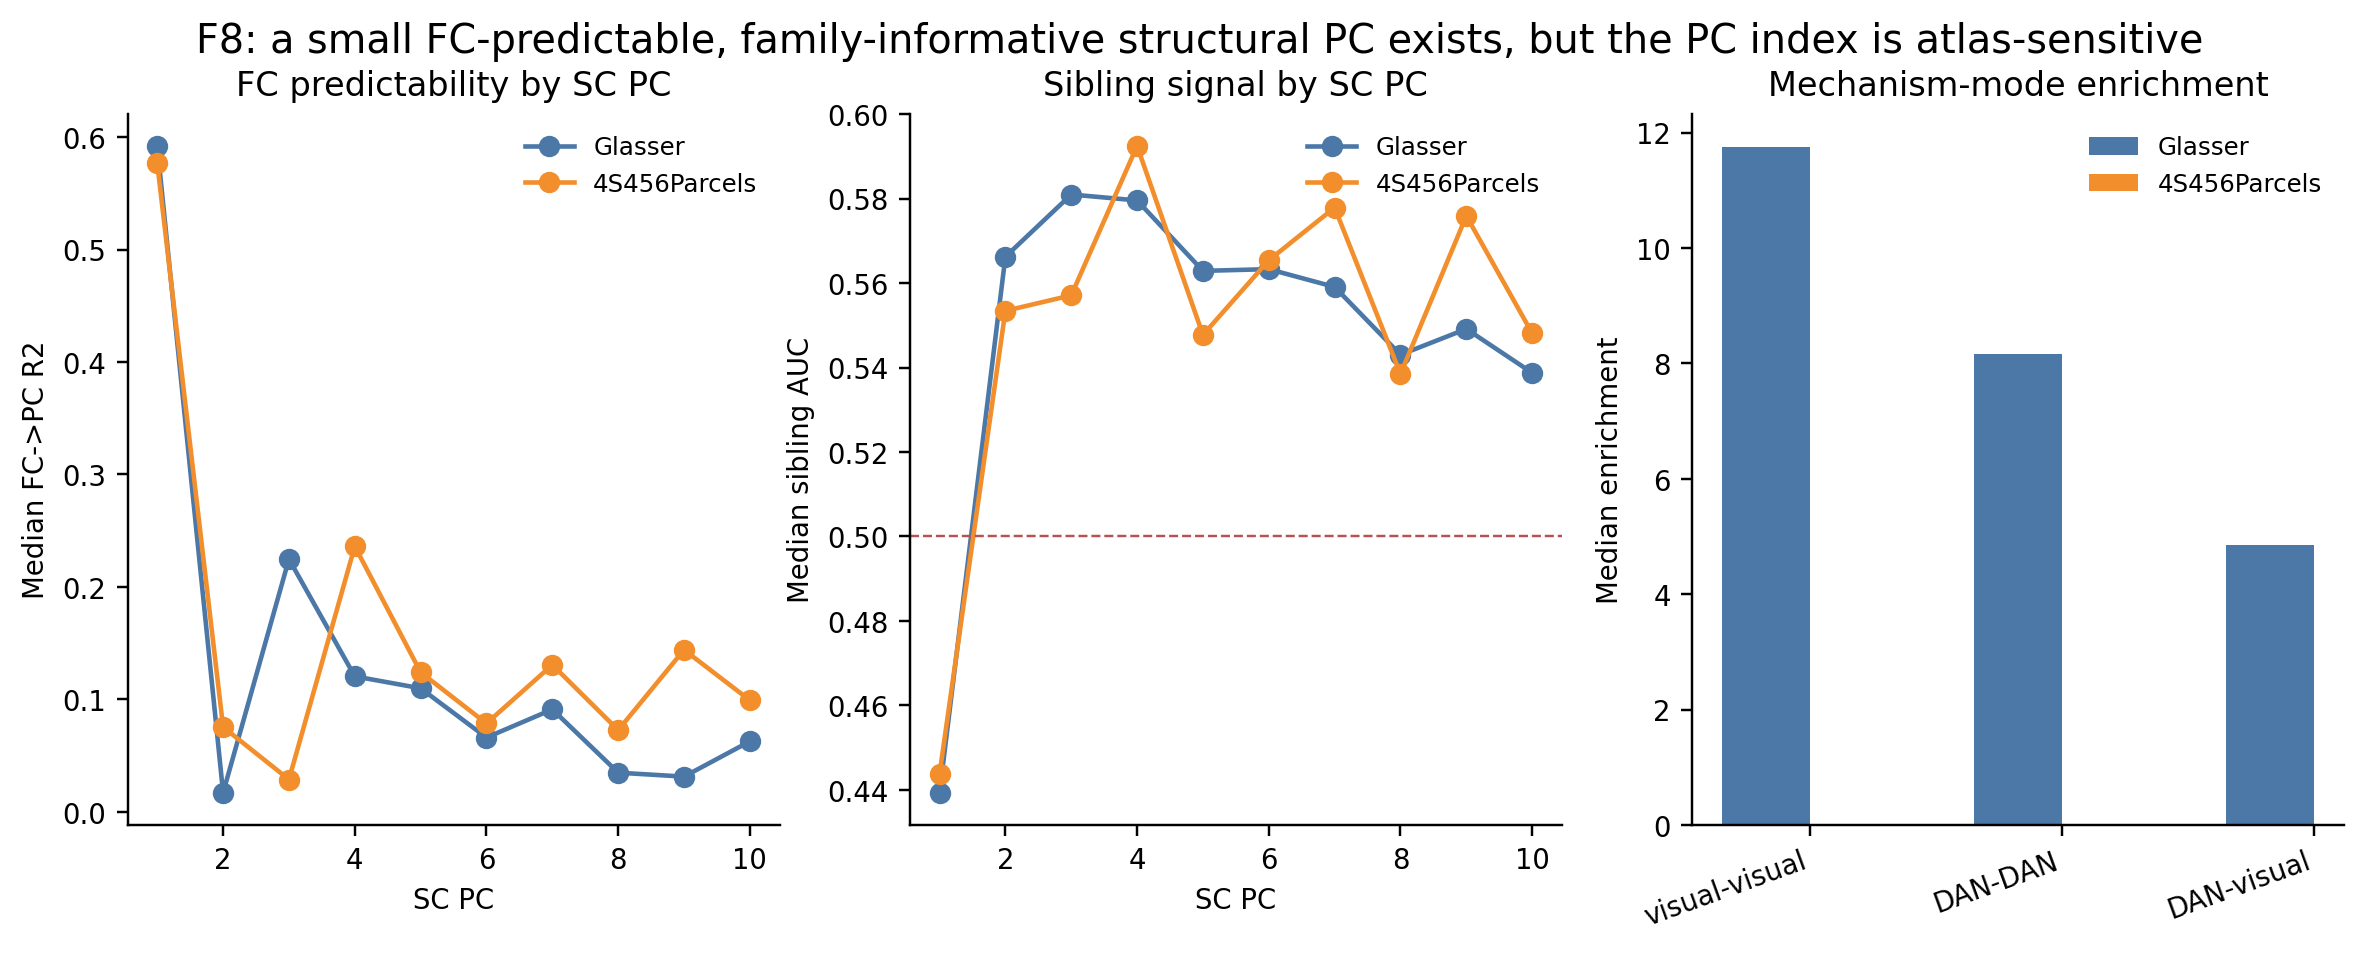
\includegraphics[width=0.95\linewidth]{figures/f8_pc_mechanism.png}
\caption{F8 mechanism ledger. FC predictability, sibling AUC, and network enrichment are shown across PCs and parcellations. The mechanism property replicates more clearly than the literal PC index.}
\label{fig:f8}
\end{figure}

\begin{table}[H]
\centering
\scriptsize
\caption{F8 PC stability, explained variance, FC predictability, and sibling AUC.}
\label{tab:f8pcs}
\begin{tabular}{llllll}
\toprule
parcellation & anchor\_pc & median\_abs\_cos & median\_expl\_var & median\_FC\_to\_PC\_R2 & median\_AUC\_sibling \\
\midrule
4S456Parcels & 1 & 0.983 & 0.038 & 0.577 & 0.444 \\
4S456Parcels & 2 & 0.966 & 0.019 & 0.075 & 0.553 \\
4S456Parcels & 3 & 0.942 & 0.015 & 0.029 & 0.557 \\
4S456Parcels & 4 & 0.914 & 0.014 & 0.236 & 0.592 \\
4S456Parcels & 5 & 0.858 & 0.012 & 0.124 & 0.548 \\
4S456Parcels & 6 & 0.845 & 0.011 & 0.079 & 0.565 \\
4S456Parcels & 7 & 0.843 & 0.010 & 0.131 & 0.578 \\
4S456Parcels & 8 & 0.766 & 0.009 & 0.073 & 0.538 \\
4S456Parcels & 9 & 0.677 & 0.009 & 0.144 & 0.576 \\
4S456Parcels & 10 & 0.451 & 0.009 & 0.099 & 0.548 \\
Glasser & 1 & 0.985 & 0.038 & 0.592 & 0.439 \\
Glasser & 2 & 0.934 & 0.016 & 0.017 & 0.566 \\
Glasser & 3 & 0.886 & 0.015 & 0.225 & 0.581 \\
Glasser & 4 & 0.896 & 0.013 & 0.120 & 0.580 \\
Glasser & 5 & 0.868 & 0.012 & 0.110 & 0.563 \\
Glasser & 6 & 0.784 & 0.011 & 0.066 & 0.563 \\
Glasser & 7 & 0.712 & 0.010 & 0.091 & 0.559 \\
Glasser & 8 & 0.756 & 0.009 & 0.035 & 0.543 \\
Glasser & 9 & 0.628 & 0.009 & 0.031 & 0.549 \\
Glasser & 10 & 0.566 & 0.009 & 0.063 & 0.539 \\
\bottomrule
\end{tabular}
\end{table}

\begin{table}[H]
\centering
\scriptsize
\caption{F8 enrichment of the mechanism mode in visual and dorsal-attention network pairs.}
\label{tab:f8enrich}
\begin{tabular}{lllll}
\toprule
parcellation & net\_pair & median\_enrichment & min\_enrichment & median\_n\_obs \\
\midrule
Glasser & dorsal attention || dorsal attention & 8.163 & 4.583 & 28.500 \\
Glasser & dorsal attention || visual & 4.861 & 4.114 & 39.000 \\
Glasser & visual || visual & 11.741 & 9.709 & 52.000 \\
\bottomrule
\end{tabular}
\end{table}

The hedging is not weakness; it is the scientific point. The analysis already caught a
single-seed false positive in an earlier PC label. V2 therefore treats F8 as a forward map
for future work rather than a load-bearing claim.  Sources: reproduction/family\_mechanism/outputs/f8\_per\_pc.csv; reproduction/family\_mechanism/outputs/f8\_stability.csv; reproduction/family\_mechanism/outputs/f8\_pc3\_enrichment\_agg.csv; reproduction/family\_mechanism/outputs/f8\_pc3\_localization.csv; notebooks-FC\_to\_SC-experimental/sanity\_checks/tract\_check/findings.md.

\section{F9: Richer Tractography Representation Does Not Help}

\textbf{Status: Glasser/exploratory, but internally strong.} F9 asks whether SC counts
are simply too crude. The answer in the current data is no. The named-bundle r2t
representation predicts FC worse than raw streamline counts, adds no marginal signal on
top of count-SC, and fails downstream cognition. This closes the most obvious "better
structural features would rescue the story" escape route for the tested representation.

\begin{figure}[H]
\centering
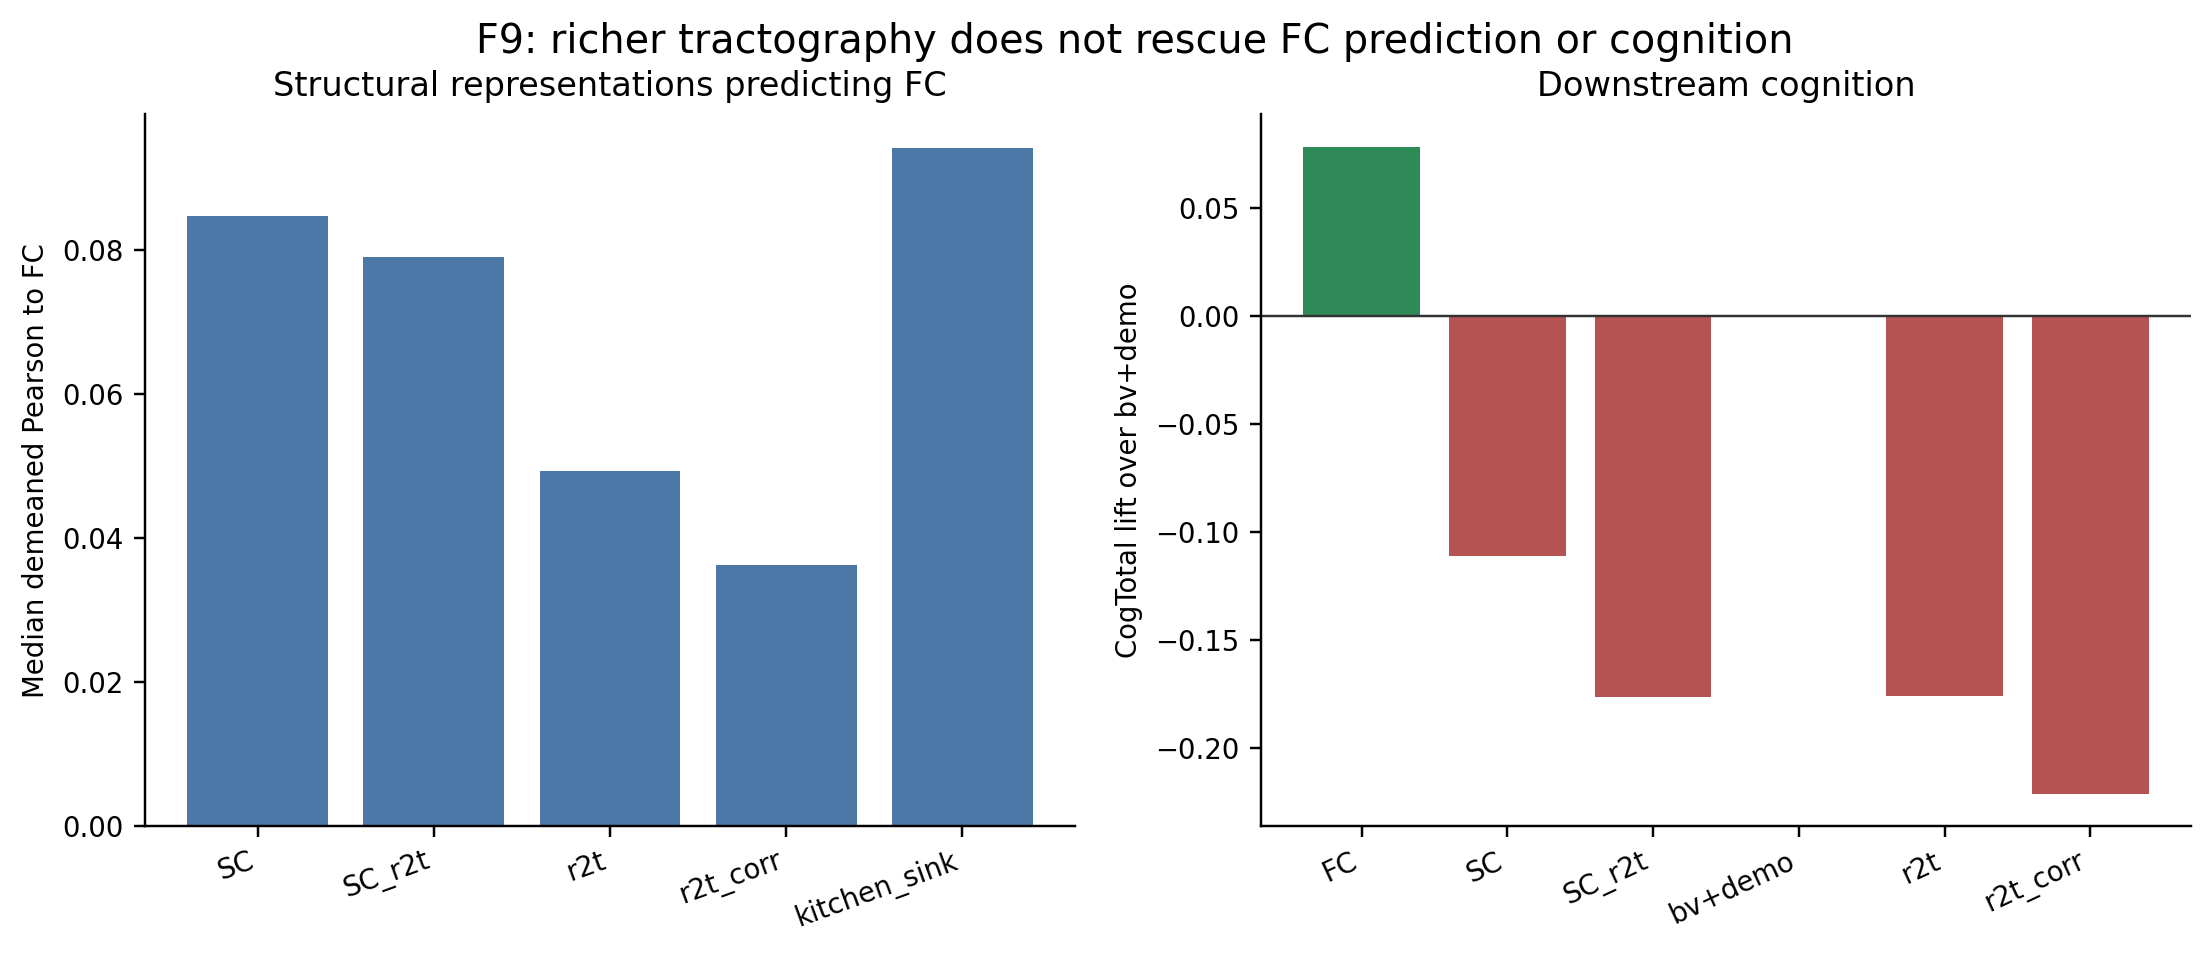
\includegraphics[width=0.95\linewidth]{figures/f9_tractography_negative.png}
\caption{F9 tractography sanity check. Count-SC beats r2t bundle features for FC prediction, and all structural/tractography representations fall below the bv+demo cognition floor.}
\label{fig:f9}
\end{figure}

\begin{table}[H]
\centering
\scriptsize
\caption{F9 source representation prediction of FC, median across seeds.}
\label{tab:f9e1}
\begin{tabular}{lllll}
\toprule
rep & demeaned\_pearson & pearson & top1\_acc & avg\_rank \\
\midrule
kitchen\_sink & 0.094 & 0.829 & 0.049 & 0.723 \\
SC & 0.085 & 0.829 & 0.051 & 0.713 \\
SC\_r2t & 0.079 & 0.827 & 0.036 & 0.702 \\
r2t & 0.049 & 0.815 & 0.021 & 0.609 \\
r2t\_corr & 0.036 & 0.823 & 0.018 & 0.607 \\
\bottomrule
\end{tabular}
\end{table}

\begin{table}[H]
\centering
\scriptsize
\caption{F9 downstream cognition for tractography representations.}
\label{tab:f9e5}
\begin{tabular}{lllll}
\toprule
rep & target & pearson\_raw & pearson\_resid & lift\_over\_bvdemo\_raw \\
\midrule
FC & CogCrystalComp\_Unadj & 0.451 & 0.374 & 0.105 \\
SC & CogCrystalComp\_Unadj & 0.267 & 0.086 & -0.079 \\
SC\_r2t & CogCrystalComp\_Unadj & 0.160 & 0.028 & -0.187 \\
bv+demo & CogCrystalComp\_Unadj & 0.346 &  & 0.000 \\
r2t & CogCrystalComp\_Unadj & 0.164 & 0.027 & -0.183 \\
r2t->synthFC & CogCrystalComp\_Unadj & 0.180 &  & -0.166 \\
r2t\_corr & CogCrystalComp\_Unadj & 0.103 & -0.009 & -0.244 \\
FC & CogFluidComp\_Unadj & 0.342 & 0.218 & 0.033 \\
SC & CogFluidComp\_Unadj & 0.180 & 0.006 & -0.130 \\
SC\_r2t & CogFluidComp\_Unadj & 0.135 & 0.072 & -0.174 \\
bv+demo & CogFluidComp\_Unadj & 0.309 &  & 0.000 \\
r2t & CogFluidComp\_Unadj & 0.130 & 0.061 & -0.179 \\
r2t->synthFC & CogFluidComp\_Unadj & 0.197 &  & -0.113 \\
r2t\_corr & CogFluidComp\_Unadj & 0.157 & 0.079 & -0.152 \\
FC & CogTotalComp\_Unadj & 0.451 & 0.264 & 0.078 \\
SC & CogTotalComp\_Unadj & 0.261 & 0.040 & -0.111 \\
SC\_r2t & CogTotalComp\_Unadj & 0.196 & 0.048 & -0.177 \\
bv+demo & CogTotalComp\_Unadj & 0.372 &  & 0.000 \\
r2t & CogTotalComp\_Unadj & 0.196 & 0.049 & -0.176 \\
r2t->synthFC & CogTotalComp\_Unadj & 0.202 &  & -0.170 \\
r2t\_corr & CogTotalComp\_Unadj & 0.151 & -0.029 & -0.221 \\
\bottomrule
\end{tabular}
\end{table}

Because F9 is Glasser-only, it should not be overclaimed as a universal tractography
result. But it is exactly the right sanity check for this preprint: richer structural
features do not recover FC's cognition signal in the tested regime.  Sources: notebooks-FC\_to\_SC-experimental/tractography\_predict/e1\_source\_rep\_results.csv; notebooks-FC\_to\_SC-experimental/tractography\_predict/e2\_asymmetry\_summary.csv; notebooks-FC\_to\_SC-experimental/tractography\_predict/e3\_marginal\_summary.csv; notebooks-FC\_to\_SC-experimental/tractography\_predict/e5\_downstream\_summary.csv; notebooks-FC\_to\_SC-experimental/tractography\_predict/findings.md.

\section{F10: Nonlinear Models and More Data Do Not Break the Ceiling}

\textbf{Status: Glasser/exploratory, but broad within that scope.} F10 closes the
"bigger model" and "more data in this regime" escape routes. Kernel ridge preserves FC's
known cognition signal but does not unlock tractography. Residual boosting gives the
nonlinear model the linear answer for free and still finds no cognition residual.
Cross-modal sink models dilute FC rather than improve it. The sample-size curve shows the
nonlinear gap does not grow into positive territory through the tested n.

\begin{figure}[H]
\centering
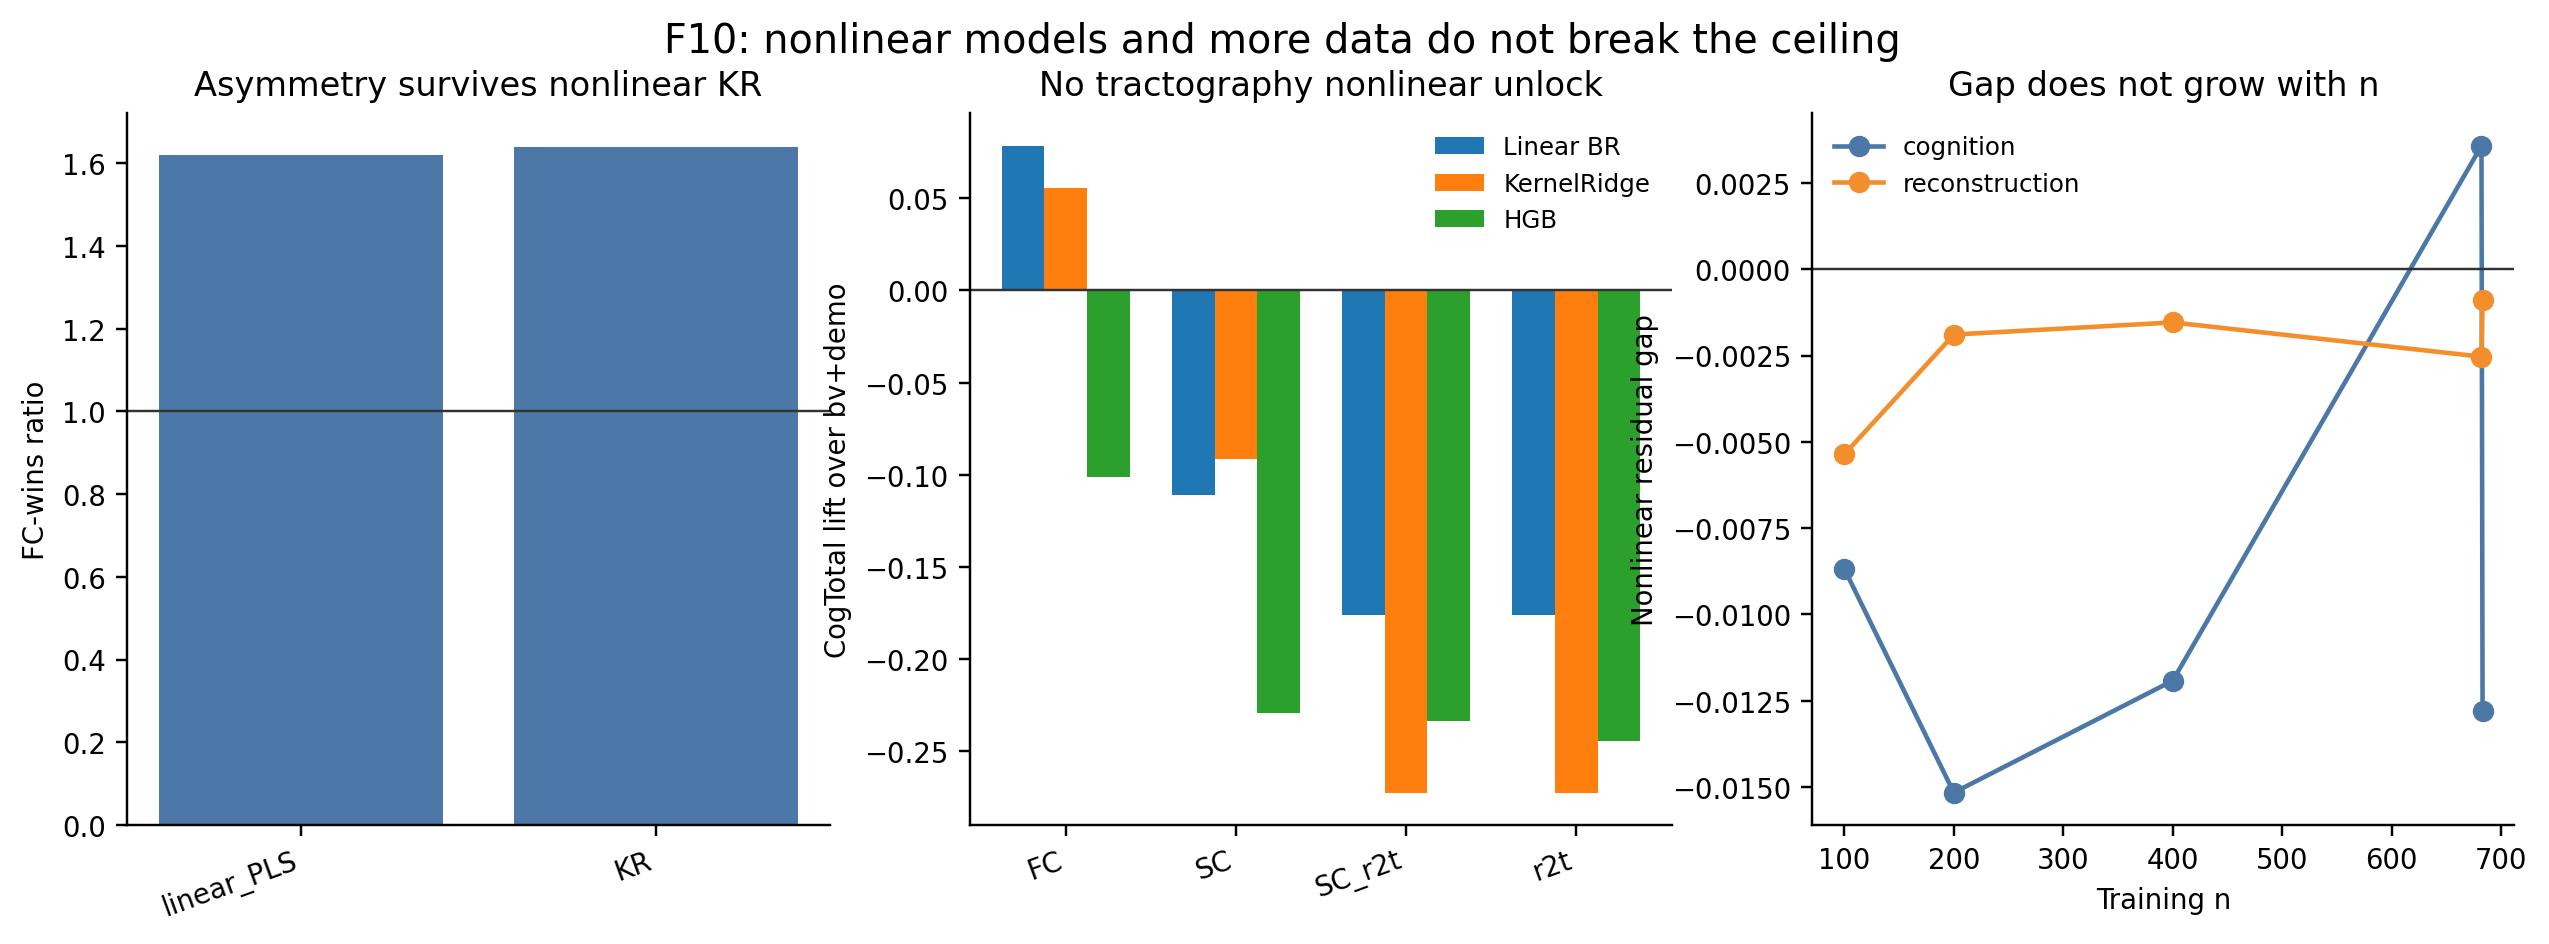
\includegraphics[width=0.95\linewidth]{figures/f10_nonlinear_scaling.png}
\caption{F10 nonlinear and scaling checks. KernelRidge preserves the asymmetry but does not unlock tractography cognition. The residual nonlinear gap stays at or below zero as n increases.}
\label{fig:f10}
\end{figure}

\begin{table}[H]
\centering
\scriptsize
\caption{F10 residual-boost reconstruction improvements. The small positive reconstruction sliver is far below the practical threshold.}
\label{tab:f10n4}
\begin{tabular}{llllll}
\toprule
rep & direction & median\_template & median\_final & median\_improvement & wilcoxon\_p\_improve \\
\midrule
SC & FC->SC & 0.135 & 0.141 & 0.005 & 9.77e-04 \\
SC & SC->FC & 0.085 & 0.087 & 0.002 & 9.77e-04 \\
r2t & FC->r2t & 0.111 & 0.117 & 0.006 & 9.77e-04 \\
r2t & r2t->FC & 0.049 & 0.053 & 0.004 & 9.77e-04 \\
r2t\_corr & FC->r2t\_corr & 0.058 & 0.062 & 0.005 & 9.77e-04 \\
r2t\_corr & r2t\_corr->FC & 0.036 & 0.040 & 0.004 & 9.77e-04 \\
\bottomrule
\end{tabular}
\end{table}

\begin{table}[H]
\centering
\scriptsize
\caption{F10 sample-size scaling summary.}
\label{tab:f10n6}
\begin{tabular}{lllllll}
\toprule
task & n\_sub & n\_seeds & median\_linear & median\_final & median\_gap & wilcoxon\_p\_gap\_gt0 \\
\midrule
cognition & 100 & 10 & 0.302 & 0.290 & -0.009 & 1.000 \\
cognition & 200 & 10 & 0.327 & 0.324 & -0.015 & 0.993 \\
cognition & 400 & 10 & 0.394 & 0.380 & -0.012 & 0.999 \\
cognition & 682 & 1 & 0.482 & 0.486 & 0.004 & 0.500 \\
cognition & 683 & 9 & 0.391 & 0.375 & -0.013 & 0.990 \\
reconstruction & 100 & 10 & 0.041 & 0.035 & -0.005 & 0.999 \\
reconstruction & 200 & 10 & 0.067 & 0.065 & -0.002 & 0.884 \\
reconstruction & 400 & 10 & 0.094 & 0.093 & -0.002 & 0.990 \\
reconstruction & 682 & 1 & 0.110 & 0.107 & -0.003 & 1.000 \\
reconstruction & 683 & 9 & 0.110 & 0.110 & -8.87e-04 & 0.980 \\
\bottomrule
\end{tabular}
\end{table}

F10 should be framed as a structural ceiling for this HCP-YA, normal-range cognition,
cross-sectional setting. It does not prove there is no signal in clinical, longitudinal,
or much larger cohorts. It does prove that the ordinary escape routes do not explain the
current null.  Sources: notebooks-FC\_to\_SC-experimental/non-linear-sanity-check/n1\_cognition\_summary.csv; notebooks-FC\_to\_SC-experimental/non-linear-sanity-check/n2\_reconstruction\_summary.csv; notebooks-FC\_to\_SC-experimental/non-linear-sanity-check/n3\_marginal\_summary.csv; notebooks-FC\_to\_SC-experimental/non-linear-sanity-check/n4\_cog\_summary.csv; notebooks-FC\_to\_SC-experimental/non-linear-sanity-check/n4\_recon\_summary.csv; notebooks-FC\_to\_SC-experimental/non-linear-sanity-check/n5\_cog\_summary.csv; notebooks-FC\_to\_SC-experimental/non-linear-sanity-check/n5\_recon\_summary.csv; notebooks-FC\_to\_SC-experimental/non-linear-sanity-check/n6\_scaling\_summary.csv; notebooks-FC\_to\_SC-experimental/non-linear-sanity-check/findings\_nonlinear.md; notebooks-FC\_to\_SC-experimental/non-linear-sanity-check/findings\_residual.md; notebooks-FC\_to\_SC-experimental/non-linear-sanity-check/findings\_scaling.md; notebooks-FC\_to\_SC-experimental/sanity\_checks/noise\_sanity\_check/findings\_noise.md.

\section{Cross-Cutting Sanity Checks}

Several sanity checks are not standalone findings but protect the ledger. The
reduction-axis analysis shows F1 is not a PCA artifact. The FC reliability analysis shows
the SC->FC gap is not explained by per-subject FC reliability. The leak verdict grid shows
zero genuine leak failures.

\begin{figure}[H]
\centering
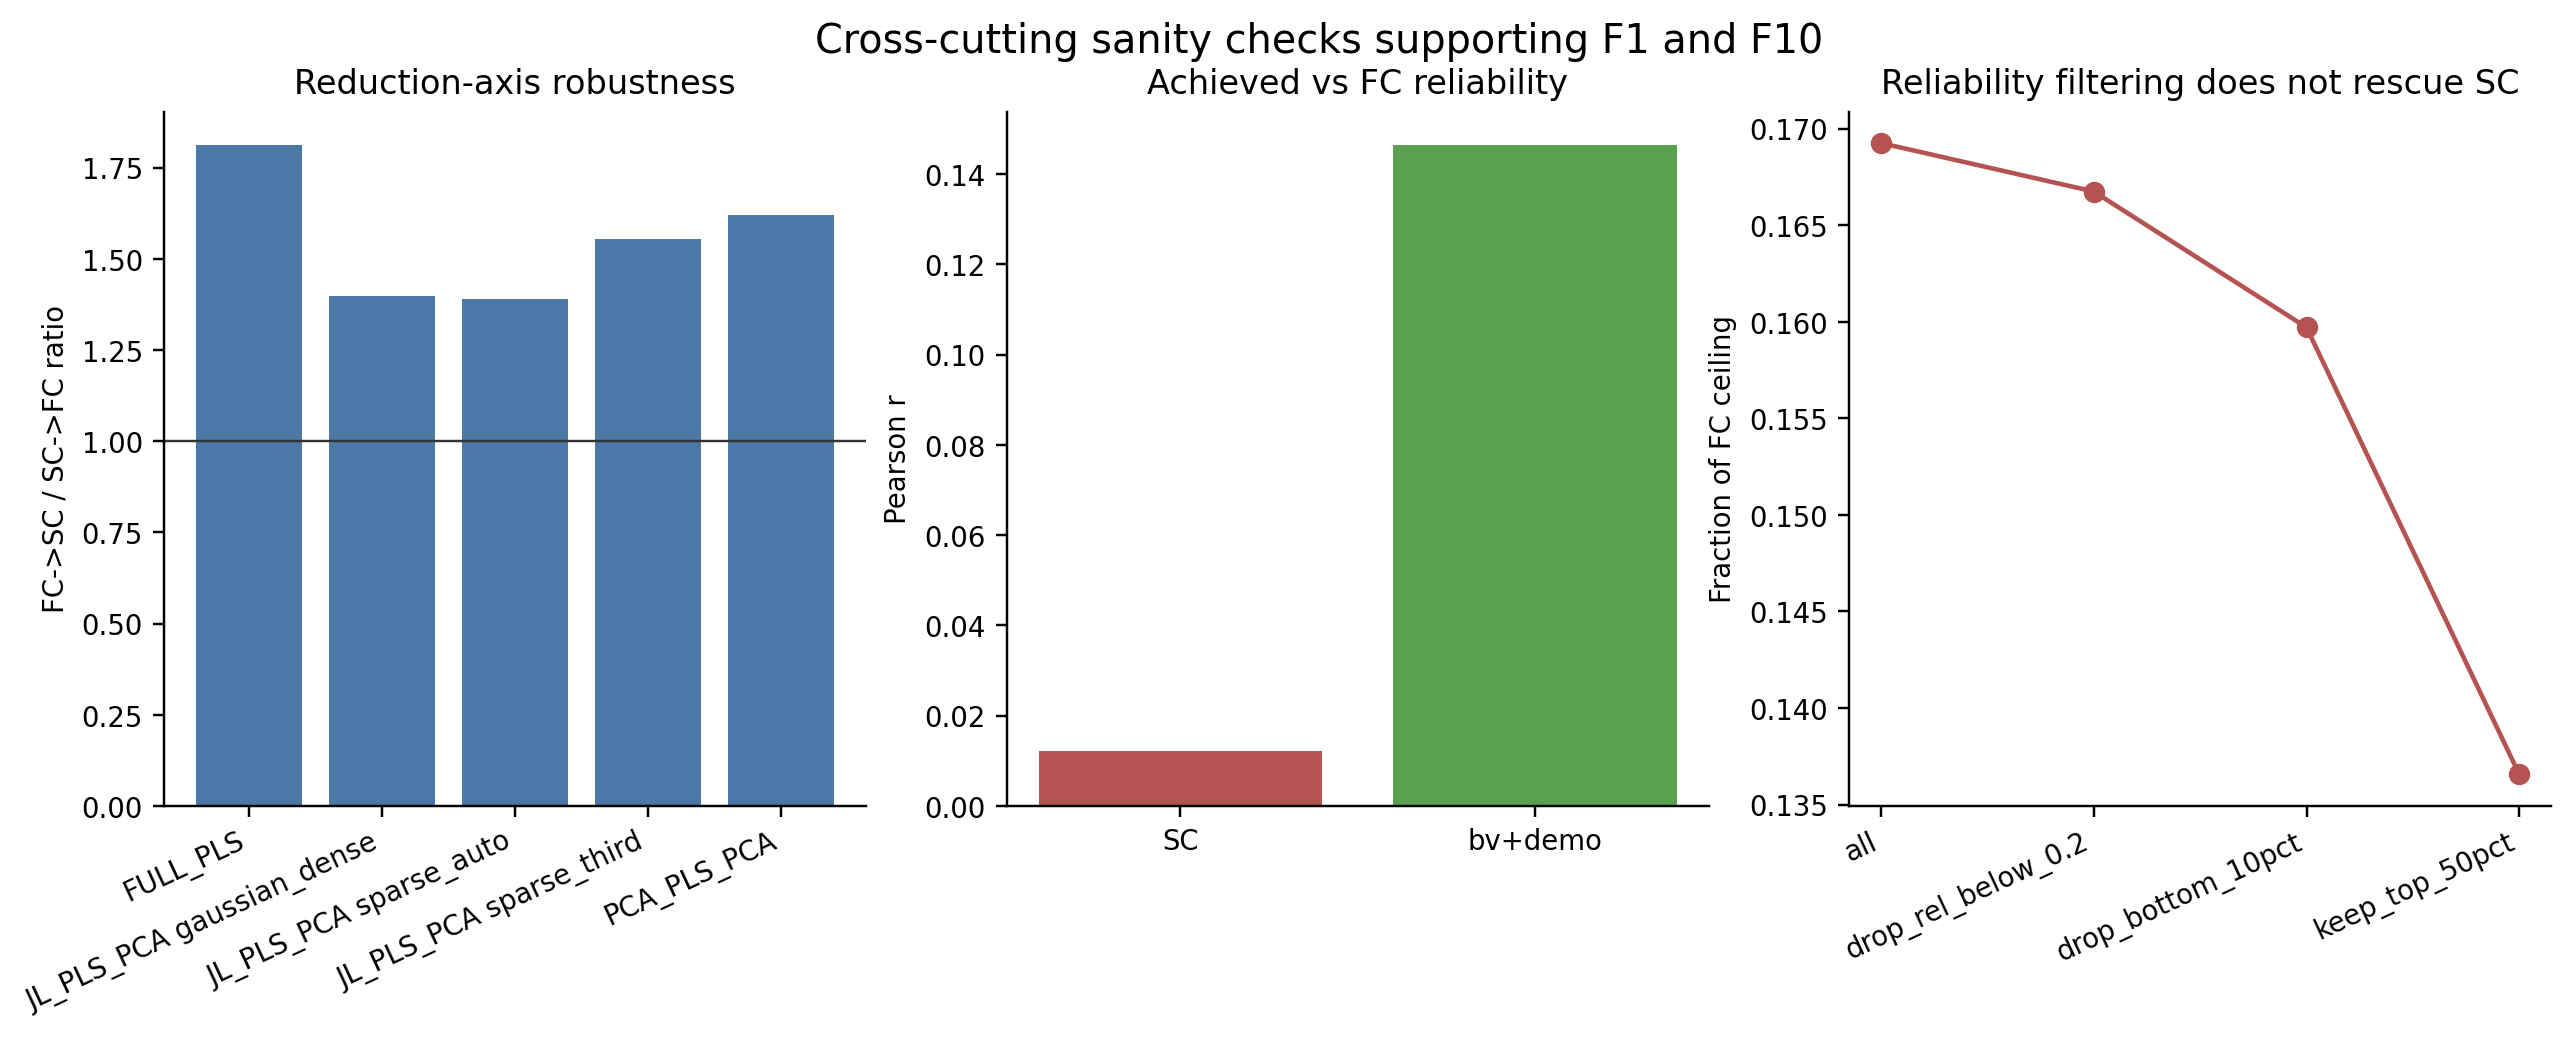
\includegraphics[width=0.95\linewidth]{figures/sanity_reduction_noise.png}
\caption{Cross-cutting sanity checks. Reduction choice preserves the F1 ratio; per-subject FC reliability does not explain SC->FC achieved performance; reliability filtering does not rescue SC.}
\label{fig:sanity}
\end{figure}

\begin{table}[H]
\centering
\scriptsize
\caption{Reduction-axis robustness supporting F1.}
\label{tab:reduction}
\begin{tabular}{lllllllll}
\toprule
method & jl\_variant & n\_seeds & median\_ratio & min\_ratio & max\_ratio & wilcoxon\_p\_vs\_1 & median\_FC\_to\_SC\_dp & median\_SC\_to\_FC\_dp \\
\midrule
FULL\_PLS &  & 10.000 & 1.813 & 1.493 & 2.115 & 9.77e-04 & 0.138 & 0.076 \\
JL\_PLS\_PCA & gaussian\_dense & 10.000 & 1.397 & 1.194 & 2.250 & 9.77e-04 & 0.084 & 0.061 \\
JL\_PLS\_PCA & sparse\_auto & 10.000 & 1.389 & 1.109 & 1.903 & 9.77e-04 & 0.084 & 0.059 \\
JL\_PLS\_PCA & sparse\_third & 10.000 & 1.554 & 1.235 & 1.776 & 9.77e-04 & 0.085 & 0.053 \\
PCA\_PLS\_PCA &  & 10.000 & 1.621 & 1.324 & 1.861 & 9.77e-04 & 0.135 & 0.085 \\
\bottomrule
\end{tabular}
\end{table}

\begin{table}[H]
\centering
\scriptsize
\caption{Per-subject FC achieved-vs-ceiling correlations supporting F10.}
\label{tab:noise}
\begin{tabular}{llllll}
\toprule
source & n & pearson\_achieved\_vs\_ceiling & pearson\_p & spearman\_achieved\_vs\_ceiling & spearman\_p \\
\midrule
SC & 857 & 0.012 & 0.722 & -9.67e-04 & 0.977 \\
bv+demo & 857 & 0.147 & 1.66e-05 & 0.147 & 1.66e-05 \\
\bottomrule
\end{tabular}
\end{table}

\section{Limitations and Exact Next Experiments}

\begin{itemize}
\item \textbf{SC-side reliability remains data-blocked.} FC reliability is well
measured, but a true SC test-retest or tractography perturbation ceiling is still needed.
\item \textbf{F9 and F10 should be ported to both parcellations.} The Glasser results
are internally coherent, but the v2 ledger should label them exploratory until the same
nonlinear/tractography checks run under 4S456Parcels.
\item \textbf{F8 needs property-selected localization.} The mechanism mode should be
selected by properties such as non-confounded FC predictability and family signal, not by
hard-coded PC index.
\item \textbf{Objective interpolation is the cleanest new experiment.} Train along a
ladder from reconstruction to cognition to fingerprint/family objectives, then ask where
the signals diverge.
\item \textbf{External validity is not solved.} HCP-YA is healthy, cross-sectional, and
normal-range cognition. The protocol should be repeated in clinical, longitudinal, or
larger cohorts with the bv+demo baseline carried along.
\end{itemize}

\section{Conclusion}

The F1--F10 ledger supports a sharper, more disciplined manuscript than the compact draft.
The data do not say that cross-modal prediction is impossible. They say that cross-modal
prediction is directional, objectively real, and biologically structured, but that
reconstruction is the wrong proxy for downstream cognition. Observed FC is the useful
cognition modality in this regime. SC and richer structural representations are valuable
for other biological questions, including family structure and mechanism hypotheses, but
they do not transfer FC's cognitive utility through imputation. The scientific redirect is
therefore concrete: report bv+demo, stop treating reconstruction as utility, and move any
future cognition claim to regimes where structural variation plausibly exceeds the healthy
young-adult floor.

\end{document}
